\documentclass[twoside,11pt]{article}

% \usepackage{blindtext}

% Any additional packages needed should be included after jmlr2e.
% Note that jmlr2e.sty includes epsfig, amssymb, natbib and graphicx,
% and defines many common macros, such as 'proof' and 'example'.
%
% It also sets the bibliographystyle to plainnat; for more information on
% natbib citation styles, see the natbib documentation, a copy of which
% is archived at http://www.jmlr.org/format/natbib.pdf

% Available options for package jmlr2e are:
%
%   - abbrvbib : use abbrvnat for the bibliography style
%   - nohyperref : do not load the hyperref package
%   - preprint : remove JMLR specific information from the template,
%         useful for example for posting to preprint servers.
%
% Example of using the package with custom options:
%
\usepackage[abbrvbib, preprint]{jmlr2e}
% \usepackage{jmlr2e}

% additional packages for the paper
% \usepackage{amsthm}
% \renewcommand\qedsymbol{$\blacksquare$}
\usepackage{amsmath}
\usepackage{amssymb}
\usepackage{amsfonts}
\usepackage{mathtools}
\usepackage{bm}

% \newtheorem{theorem}{Theorem}
% \newtheorem{assumption}{Assumption}
% \newtheorem{lemma}{Lemma}
% \newtheorem{proposition}{Proposition}
% \newtheorem{definition}{Definition}
% \newtheorem{corollary}{Corollary}

% \newcommand{\definitionautorefname}{Definition}
% \newcommand{\assumptionautorefname}{Assumption}
% \newcommand{\lemmaautorefname}{Lemma}
% \newcommand{\propositionautorefname}{Proposition}

% \usepackage{multirow}

% \usepackage{setspace}
% \setstretch{1}

% \usepackage{natbib}


% \usepackage{colortbl} 

% define useful colors
\usepackage[table,xcdraw]{xcolor}
% 
\definecolor{cambridgeblue}{RGB}{163, 193, 173}
% 
\definecolor{CambridgeSuperLightBlue}{RGB}{204, 227, 245}
\definecolor{CambridgeSuperLightOrange}{RGB}{252, 229, 205}
\definecolor{CambridgeSuperLightPurple}{RGB}{142,37,141}
\definecolor{CambridgeSuperLightGreen}{RGB}{217, 234, 211}
% 
\definecolor{CambridgeDarkLightBlue}{RGB}{84,138,182}
\definecolor{CambridgeLightBlue}{RGB}{106,173,228}
\definecolor{CambridgeLightOrange}{RGB}{239,189,71}
\definecolor{CambridgeLightGreen}{RGB}{168,180,0}
\definecolor{CambridgeLightPurple}{RGB}{181,147,155}
\definecolor{CambridgeLightTeal}{RGB}{163,193,173}
% 
\definecolor{CambridgeCoreBlue}{RGB}{0,115,207}
\definecolor{CambridgeCoreOrange}{RGB}{227,114,34}
\definecolor{CambridgeCoreBurgundy}{RGB}{144,27,59}
\definecolor{CambridgeCoreGreen}{RGB}{88,166,24}
\definecolor{CambridgeCorePurple}{RGB}{142,37,141}
\definecolor{CambridgeCoreTeal}{RGB}{0,179,190}
% 
\definecolor{CambridgeDarkBlue}{RGB}{0,62,114}
\definecolor{CambridgeDarkOrange}{RGB}{200,78,0}
\definecolor{CambridgeDarkGreen}{RGB}{67,81,37}
\definecolor{CambridgeDarkPurple}{RGB}{65,45,93}
\definecolor{CambridgeDarkTeal}{RGB}{21,101,112}
% 
\definecolor{CambridgeWhitePrint}{RGB}{255,255,255}
\definecolor{CambridgeBlackPrint}{RGB}{0,0,0}
% 
\definecolor{CambridgeYellow}{RGB}{220,20,6}

\definecolor{mygrey}{RGB}{170, 170, 170}
\definecolor{mylightgrey}{RGB}{230, 230, 230}


% % \usepackage[shortlabels]{enumitem}
% \renewcommand{\labelenumi}{(\theenumi)}

% \usepackage[parfill]{parskip}
% \setlength{\parskip}{10pt}


% \renewcommand\labelitemi{--}


% \usepackage{titlesec}
% % numbering of \paragraph like \subsubsubsection
% \setcounter{secnumdepth}{4}
% \titleformat{\paragraph}
% {\normalfont\normalsize\bfseries}{\theparagraph}{1em}{}
% \titlespacing*{\paragraph}
% {0pt}{3.25ex plus 1ex minus .2ex}{1.5ex plus .2ex}


\usepackage{tikz}
\usetikzlibrary{automata, positioning, arrows.meta, decorations.markings, calc}
\tikzset{
    middle arrow/.style={
        decoration={markings,
            mark=at position #1 with {\arrow{>}}}, % Choose arrow style here
        postaction={decorate},
        thick
    }
}


% % \newcommand\drawsteparrow[5]{
% %     % Extract start and end coordinates
% %     \coordinate (start) at (#1,#2);
% %     \def\xstart{#1}
% %     \def\ystart{#2}
% %     \def\xend{#3}
% %     \def\yend{#4}
% %     % Number of steps
% %     \def\numsteps{#5}
    
% %     % Calculate step sizes
% %     \pgfmathsetmacro{\xstep}{(\xend - \xstart)/(\numsteps/2)}
% %     \pgfmathsetmacro{\ystep}{(\yend - \ystart)/(\numsteps/2)}
    
% %     % Initialize current position
% %     \coordinate (current) at (start);
    
% %     % Loop to draw steps
% %     \foreach \i in {1,...,\numsteps} {
% %         \ifnum\i=\numexpr\numsteps/2+1\relax
% %             \draw[
% %                 decoration={
% %                     markings,
% %                     mark=at position 0.5 with {\arrow{>}},
% %                 },
% %                 postaction={decorate},
% %                 thick
% %             ] (current) -- ++((mod(\i,2)*\xstep,(1-mod(\i,2))*\ystep)) coordinate (current);
% %         \else
% %             \draw[thick] (current) -- ++((mod(\i,2)*\xstep,(1-mod(\i,2))*\ystep)) coordinate (current);
% %         \fi
% %     }
% % }


% % Load hyperref package with custom link colors and without boxes
% \usepackage[
%     colorlinks=true,       % Enable colored links
%     linkcolor=CambridgeCoreBlue,  % Color for internal links (e.g., sections, pages)
%     citecolor=CambridgeCoreBlue,  % Color for citations
%     urlcolor=CambridgeCoreBlue,   % Color for URLs
%     filecolor=CambridgeCoreBlue,  % Color for files
%     linkbordercolor={0 0 0},  % Black for link border (invisible)
%     citebordercolor={0 0 0},  % Black for citation border (invisible)
%     urlbordercolor={0 0 0}    % Black for URL border (invisible)
% ]{hyperref}


\usepackage{aliascnt}


% % Define a custom theorem style with non-italic text
% \newtheoremstyle{nonItalic}%
% {}   % Space above
% {}   % Space below
% {\upshape}  % Body font
% {}          % Indent amount
% {\bfseries} % Theorem head font % \sffamily
% {}         % Punctuation after theorem head
% {\newline}         % Space after theorem head
% {}          % Theorem head spec (can be left empty, meaning `normal`)

% % use frames
% \usepackage{mdframed}
% \mdfdefinestyle{thmstyle}{%
%     % line
%     linecolor = black,
%     linewidth = 0.5 pt,
%     topline=true,     % Show top border
%     bottomline=true,  % Show bottom border
%     leftline=true,   % Hide left border
%     rightline=true,  % Hide right border
%     % middlelinewidth=2pt,
%     roundcorner = 10 pt,
%     % background
%     backgroundcolor = white,
%     % frametitlebackgroundcolor= mygrey!20,
%     % margins
%     leftmargin = 0,
%     rightmargin = 0,
%     innerbottommargin = \topskip ,
%     innertopmargin = \topskip,
%     innerleftmargin = \topskip ,
%     innerrightmargin = \topskip,
%     % splittopskip = \topskip ,
%     skipabove = \topskip ,
%     skipbelow = \topskip ,
%     % ntheorem = true,
%     % frame title
%     % frametitlerule=true,
%     % frametitlefont= \bfseries, %\sffamily
% }

% % Apply the new non-italic style to the theorem environments
% \theoremstyle{nonItalic}
% \newtheorem{parentthm}{Theorem}
% \numberwithin{parentthm}{section}
% \numberwithin{figure}{section}

% \newaliascnt{theorem}{parentthm}
% \newmdtheoremenv[style=thmstyle]{theorem}[theorem]{Theorem}
% \aliascntresetthe{theorem}
% \renewcommand{\theHtheorem}{theorem.\thesection.\thetheorem}
% \renewcommand{\theoremautorefname}{Theorem}

% \newaliascnt{assumption}{parentthm}
% \newmdtheoremenv[style=thmstyle]{assumption}[assumption]{Assumption}
% \aliascntresetthe{assumption}
% \renewcommand{\theHassumption}{assumption.\thesection.\theassumption}
% \newcommand{\assumptionautorefname}{Assumption}

% \newaliascnt{proposition}{parentthm}
% \newmdtheoremenv[style=thmstyle]{proposition}[proposition]{Proposition}
% \aliascntresetthe{proposition}
% \renewcommand{\theHproposition}{proposition.\thesection.\theproposition}
% \newcommand{\propositionautorefname}{Proposition}

% \newaliascnt{lemma}{parentthm}
% \newmdtheoremenv[style=thmstyle]{lemma}[lemma]{Lemma}
% \aliascntresetthe{lemma}
% \renewcommand{\theHlemma}{lemma.\thesection.\thelemma}
% \newcommand{\lemmaautorefname}{Lemma}

% \newaliascnt{conjecture}{parentthm}
% \newmdtheoremenv[style=thmstyle]{conjecture}[conjecture]{Conjecture}
% \aliascntresetthe{conjecture}
% \renewcommand{\theHconjecture}{conjecture.\thesection.\theconjecture}
% \newcommand{\conjectureautorefname}{Conjecture}

% \newaliascnt{corollary}{parentthm}
% \newmdtheoremenv[style=thmstyle]{corollary}[corollary]{Corollary}
% \aliascntresetthe{corollary}
% \renewcommand{\theHcorollary}{corollary.\thesection.\thecorollary}
% \newcommand{\corollaryautorefname}{Corollary}

% \newaliascnt{definition}{parentthm}
% \newmdtheoremenv[style=thmstyle]{definition}[definition]{Definition}
% \aliascntresetthe{definition}
% \renewcommand{\theHdefinition}{definition.\thesection.\thedefinition}
% \newcommand{\definitionautorefname}{Definition}

% \newaliascnt{example}{parentthm}
% \newmdtheoremenv[style=thmstyle]{example}[example]{Example}
% \aliascntresetthe{example}
% \renewcommand{\theHexample}{example.\thesection.\theexample}
% \newcommand{\exampleautorefname}{Example}

% \newaliascnt{remark}{parentthm}
% \newmdtheoremenv[style=thmstyle]{remark}[remark]{Remark}
% \aliascntresetthe{remark}
% \renewcommand{\theHremark}{remark.\thesection.\theremark}
% \newcommand{\remarkautorefname}{Remark}

% \newaliascnt{claim}{parentthm}
% \newmdtheoremenv[style=thmstyle]{claim}[claim]{Claim}
% \aliascntresetthe{claim}
% \renewcommand{\theHclaim}{claim.\thesection.\theclaim}
% \newcommand{\claimautorefname}{Claim}

% \newaliascnt{algorithm}{parentthm}
% \newmdtheoremenv[style=thmstyle]{algorithm}[algorithm]{Algorithm}
% \aliascntresetthe{algorithm}
% \renewcommand{\theHalgorithm}{algorithm.\thesection.\thealgorithm}
% \newcommand{\algorithmautorefname}{Algorithm}

% \newaliascnt{property}{parentthm}
% \newmdtheoremenv[style=thmstyle]{property}[property]{Property}
% \aliascntresetthe{property}
% \renewcommand{\theHproperty}{property.\thesection.\theproperty}
% \newcommand{\propertyautorefname}{Property}

% \newaliascnt{notation}{parentthm}
% \newmdtheoremenv[style=thmstyle]{notation}[notation]{Notation}
% \aliascntresetthe{notation}
% \renewcommand{\theHnotation}{notation.\thesection.\thenotation}
% \newcommand{\notationautorefname}{Notation}

% % use to do notes
% \usepackage[colorinlistoftodos, textsize=scriptsize, textwidth=3.3cm]{todonotes}
% \newcommand{\mytodo}[1]{\todo[linecolor=CambridgeCoreOrange,backgroundcolor=CambridgeSuperLightOrange,bordercolor=CambridgeCoreOrange]{\textcolor{CambridgeCoreOrange}{#1}}}

% \usepackage{graphicx}
\usepackage{subcaption}
\usepackage{caption}
% \captionsetup[figure]{labelfont=bf}
% \captionsetup[table]{labelfont=bf}

\usepackage{pgfplots}
\usepgfplotslibrary{groupplots}
\pgfplotsset{compat=1.18}

% \usepackage{pgfplotstable}
% \usepgfplotslibrary{fillbetween}

\usepackage{float}

\usepackage{enumitem}
\usepackage{microtype}
\renewenvironment{proof}[1][Proof]
  {\par\noindent{\bfseries #1.}\quad}
  {\unskip\nobreak\hfill\penalty50\hskip1em\null\nobreak\hfill
   \BlackBox\par\vspace{2mm}}

% \usepackage{bm}
% \usepackage{amsmath}
% \usepackage{aliascnt}
% Fix Definition from jmlr2e
\let\definition\relax
\let\enddefinition\relax
\newaliascnt{definition}{theorem}
\newtheorem{definition}[definition]{Definition}
\aliascntresetthe{definition}
\providecommand*{\definitionautorefname}{Definition}

% Add Assumption
\newaliascnt{assumption}{theorem}
\newtheorem{assumption}[assumption]{Assumption}
\aliascntresetthe{assumption}
\providecommand*{\assumptionautorefname}{Assumption}

\let\lemma\relax
\let\endlemma\relax
\newaliascnt{lemma}{theorem}
\newtheorem{lemma}[lemma]{Lemma}
\aliascntresetthe{lemma}
\providecommand*{\lemmaautorefname}{Lemma}

\let\proposition\relax
\let\endproposition\relax
\newaliascnt{proposition}{theorem}
\newtheorem{proposition}[proposition]{Proposition}
\aliascntresetthe{proposition}
\providecommand*{\propositionautorefname}{Proposition}

% Definitions of handy macros can go here
% words
\newcommand{\rlL}{reinforcement learning}
% \newcommand{\RlL}{Reinforcement learning}
\newcommand{\rlS}{RL}
\newcommand{\mlL}{machine learning}
% \newcommand{\MlL}{Machine learning}
\newcommand{\mlS}{ML}
\newcommand{\aiL}{artificial intelligence}
% \newcommand{\AiL}{Artificial intelligence}
\newcommand{\aiS}{AI}
\newcommand{\mdpL}{Markov decision process}
\newcommand{\mdpS}{MDP}
\newcommand{\mcL}{Monte Carlo}
\newcommand{\mcS}{MC}
\newcommand{\mcesL}{\mcL~exploring starts}
\newcommand{\mcesS}{MCES}
\newcommand{\mctsL}{\mcL~tree search}
\newcommand{\mctsS}{MCTS}


% loops
\newcommand{\nloopN}[0]{_{n=1}^{N}}
\newcommand{\nloopInf}[0]{_{n=1}^{\infty}}
\newcommand{\kloopK}[0]{_{k=1}^{K}}
\newcommand{\kloopInf}[0]{_{k=1}^{\infty}}

% sets
\newcommand{\states}{\mathbb{S}}
\newcommand{\actions}{\mathbb{A}}
\newcommand{\mdp}{\mathcal{M}}
\newcommand{\modmdp}{\hat{\mdp}}
\newcommand{\xset}{\mathcal{X}}
\newcommand{\kset}{\mathcal{K}}
\newcommand{\qset}{\mathcal{Q}}
\newcommand{\vset}{\mathcal{V}}
\newcommand{\aset}{\mathcal{A}}
\newcommand{\sset}{\mathcal{S}}
\newcommand{\ssetA}{\mathcal{S}^\mathsf{A}}
\newcommand{\ssetT}{\mathcal{S}^\mathsf{T}}
% \newcommand{\hist}{\mathcal{H}}
\newcommand{\polset}{\mathcal{P}}
\newcommand{\updateset}{\mathcal{M}}
\newcommand{\greedyset}{\mathcal{P}}
\newcommand{\real}{\mathbb{R}}
\newcommand{\integers}{\mathbb{Z}}
\newcommand{\naturals}{\mathbb{N}}
\newcommand{\realpos}{\mathbb{R}^+}
% \newcommand{\simplex}{\mathbb{P}}
\newcommand{\region}{\graval}
% \newcommand{\episode}{\mathcal{E}}
\newcommand{\hist}{\mathcal{F}}
\newcommand{\ball}{\mathcal{B}}
% \DeclareMathOperator{\updateset}{\mathsf{M}}
% \DeclareMathOperator{\avalset}{\mathsf{Q}}

% functions
\newcommand{\saprior}{\update_0}
\newcommand{\transit}{\tau}
% \newcommand{\modtransprob}{{\hat{p}_\T}}
\newcommand{\pol}{\pi}
\newcommand{\update}{\mu}
\newcommand{\start}{\sigma}
\newcommand{\bias}{b}
\newcommand{\qval}{q}
\newcommand{\sval}{v}
\newcommand{\aval}{a}
\newcommand{\step}{\delta}
% \newcommand{\pol}{{\mathsf{\pi}}}
% \newcommand{\update}{\mathsf{p}}
% \newcommand{\aval}{\mathsf{q}}
% \newcommand{\pol}{{\bm{\pi}}}
% \newcommand{\update}{\bm{p}}
% \newcommand{\aval}{\bm{q}}
% \newcommand{\sval}{\bm{v}}
% \newcommand{\updateold}{p\polold}
\newcommand{\transprobmat}{\T}
\newcommand{\reward}{r}
\newcommand{\sterm}{s_T}
\newcommand{\qpol}{\qval_\pol}
\newcommand{\qopt}{\qval_{\best{\pol}}}
% \newcommand{\qopt}{\best{q}}

% \newcommand{\modpol}{\hat{\pol}}
% \newcommand{\modbellq}{\hat{\bellq}}
\newcommand{\onefun}{\mathbf{1}}
% \newcommand{\ones}{\mathbf{1}}
\newcommand{\zerofun}{\mathbf{0}}

\newcommand{\grpol}{P}
\newcommand{\graval}{Q}

% numbers
\newcommand{\discount}{\gamma}
\newcommand{\lrate}{\alpha}
\newcommand{\diff}{\mathrm{d}}
\newcommand{\deriv}[2]{\dfrac{\diff #1}{\diff #2}}
\newcommand{\pderiv}[2]{\dfrac{\partial #1}{\partial #2}}
\newcommand{\blambda}{\bm{\lambda}}

% vectors
\newcommand{\bv}{\mathbf{v}}
\newcommand{\bq}{\mathbf{q}}
\newcommand{\br}{\mathbf{r}}
\newcommand{\bx}{\mathbf{x}}
\newcommand{\by}{\mathbf{y}}
\newcommand{\bp}{\mathbf{p}}
\newcommand{\bone}{\mathbf{1}}


% matrices
\newcommand{\bA}{\mathbf{A}}
\newcommand{\bPi}{\Pi}
\newcommand{\bT}{\mathbf{T}}
\newcommand{\eye}{\mathbf{I}}
\newcommand{\bnull}{\mathbf{0}}
\newcommand{\bW}{\mathbf{W}}

% expressions
% \DeclareMathOperator*{\E}{\mathbb{E}}
% % \newcommand{\expect}[1]{{\mathbb{E}[#1]}}
% % \newcommand{\expectB}[1]{{\mathbb{E}\Big[#1\Big]}}
% % \newcommand{\expectpol}[2]{{\mathbb{E}_{#1}[#2}}
% \DeclareMathOperator*{\prob}{\mathbb{P}}
% % \newcommand{\prob}[1]{{\mathbb{P}[#1]}}
% % \newcommand{\probB}[1]{{\mathbb{P}\Big[#1\Big]}}
% \DeclareMathOperator{\B}{\mathsf{B}}
% \DeclareMathOperator{\I}{\mathsf{I}}
% \DeclareMathOperator{\Pol}{\mathsf{P}}
% \DeclareMathOperator{\T}{\mathsf{T}}
% \DeclareMathOperator*{\conv}{\textup{conv}}
% \DeclareMathOperator*{\convex}{\textup{conv}}
% \DeclareMathOperator*{\argmax}{argmax}
% \DeclareMathOperator*{\argmin}{argmin}
% % \DeclareMathOperator*{\limsup}{limsup}
% % \DeclareMathOperator*{\liminf}{liminf}

\newcommand{\tor}{\text{or}}
\newcommand{\tand}{\text{and}}
\newcommand{\tfor}{\text{for}}

% equations
% \newcommand{\synchrodiscrete}{
%     q\new = (1-\lrate\old \upprobold) q\old + \lrate\old  \upprobold (q\polold + v\old) \qquad \textup{for } q\old \in \region(\pol\old)
% }
% \newcommand{\synchrocontinuous}{
%     \Dot{q} = \upprob (q_\pol - q) \qquad \textup{for } q \in \region(\pol)
%     }
% \newcommand{\asynchrodiscrete}{
%     q\new(\sa) = 
%     \begin{cases}
%     (1-\lrate\old) q\old(\sa) + \lrate\old(q\polold(\sa) + w\old(\sa)) \\
%     \hfill \text{with probability } \upprobold(\sa),\\
%     q\old(\sa) \hfill \text{otherwise}.
%     \end{cases}
% }
\newcommand{\DiscreteDeterministic}[1][\update_\pol]{
    q_+ = q + \lrate f
    \ \text{with} \
    f \in F(q) \coloneqq \big\{ \ #1 ( \qpol - q ) : \pol \in \greedyset(q) \ \big\}
}
\newcommand{\DiscreteStochastic}[1][\update_\pol]{
    q_+ = q + \lrate ( f + w )
    \ \text{with} \
    f \in F(q) \coloneqq \big\{ \ #1 ( \qpol - q ) : \pol \in \greedyset(q) \ \big\}
}
\newcommand{\DifferentialInclusion}[1][\update_\pol]{
    \Dot{q} 
    \in \conv\big[F(q)\big] 
    = \conv_{\pol \in \greedyset(q)} \big[ \ #1 ( \qpol - q ) \ \big]
}

% \newcommand{\best}[1]{\smash{\overset{\scriptstyle\ast}{#1}}} %{\overline{#1}}
\newcommand{\worst}[1]{\overline{#1}} %{\underline{#1}}
\newcommand{\best}[1]{{#1}_*}
% \newcommand{\worst}[1]{\check{#1}}
% \newcommand{\best}[1]{\overset{*}{#1}}
% \newcommand{\worst}[1]{\overline{#1}}
\newcommand{\opt}{{^{\star}}}
\newcommand{\bad}{{_{-}}}
% \newcommand{\start}{[0]}
% \newcommand{\new}{[\kpo]}
% \newcommand{\old}{[\kpn]}
% \newcommand{\oldi}{[i]}
% \newcommand{\oldK}{[K]}
% \newcommand{\start}{{_0}}
\newcommand{\new}{{_\kpo}}
\newcommand{\old}{{_\kpn}}
\newcommand{\oldi}{{_\ipn}}
\newcommand{\oldK}{{_K}}

\newcommand{\polold}{{_{\pol\old}}}

\newcommand{\ipo}{{{i+1}}}
\newcommand{\imo}{{{i-1}}}
\newcommand{\imn}{{{i-n}}}
\newcommand{\ipn}{{i}}

\newcommand{\npo}{{{n+1}}}
\newcommand{\nmo}{{{n-1}}}
% \newcommand{\nmn}{{{i-n}}}
\newcommand{\npn}{{n}}

\newcommand{\mpo}{{{m+1}}}
\newcommand{\mmo}{{{m-1}}}
% \newcommand{\mmn}{{{m-n}}}
\newcommand{\mpn}{{m}}

\newcommand{\kpo}{{{k+1}}}
\newcommand{\kmo}{{{k-1}}}
\newcommand{\kpn}{{{k+n}}}
\newcommand{\kmn}{{{k-n}}}
\newcommand{\kpz}{{k}}
\newcommand{\kpN}{{{k+N}}}

\newcommand{\tpo}{{{t+1}}}
\newcommand{\tpt}{{{t+2}}}
\newcommand{\tmo}{{{t-1}}}
\newcommand{\tmn}{{{t-n}}}
\newcommand{\tpn}{{t+n}}
\newcommand{\tpnmo}{{\tpn-1}}
\newcommand{\tpnpo}{{\tpn+1}}
\newcommand{\tpk}{{t+k}}
\newcommand{\tpkmo}{{\tpk-1}}
\newcommand{\tpkpo}{{\tpk+1}}
\newcommand{\tpnpk}{{t+n+k}}
\newcommand{\tpnpkmo}{{\tpnpk-1}}
\newcommand{\tpnpkpo}{{\tpnpk+1}}

\newcommand{\lpo}{{{(l+1)}}}
\newcommand{\lmo}{{{(l-1)}}}
\newcommand{\lpn}{(l)}

\newcommand{\sat}{{{s_t,a_t}}}
\newcommand{\satpo}{{{s_\tpo,a_\tpo}}}
\newcommand{\satpt}{{{s_\tpt,a_\tpt}}}
\newcommand{\satmo}{{{s_\tmo,a_\tmo}}}
\newcommand{\satmn}{{{s_\tmn,a_\tmn}}}
\newcommand{\satpn}{{s_\tpn,a_\tpn}}
\newcommand{\satpnmo}{{s_\tpnmo,a_\tpnmo}}
\newcommand{\satpnpo}{{s_\tpnpo,a_\tpnpo}}
\newcommand{\satpk}{{s_\tpk,a_\tpk}}
\newcommand{\satpkmo}{{s_\tpkmo,a_\tpkmo}}
\newcommand{\satpkpo}{{s_\tpkpo,a_\tpkpo}}
\newcommand{\satpnpk}{{s_\tpnpk,a_\tpnpk}}
\newcommand{\satpnpkmo}{{s_\tpnpkmo,a_\tpnpkmo}}
\newcommand{\satpnpkpo}{{s_\tpnpkpo,a_\tpnpkpo}}
\newcommand{\sa}{{s,a}}
\newcommand{\sazero}{{s_0,a_0}}
\newcommand{\saT}{{s_T,a_T}}
\newcommand{\saTmo}{{{s_{T-1},a_{T-1}}}}

\newcommand{\diag}{\textup{diag}}
\newcommand{\inv}{^{-1}}
% \newcommand{\greedy}{\textup{greedy}}
\newcommand{\tri}{\bigtriangleup}
\newcommand{\block}{\square}
\newcommand{\satis}{\;:\;}
% \newcommand{\Expect}{\mathbb{E}}
% \newcommand{\greedy}{\textup{greedy}}
\newcommand{\interior}{\textup{int} \,}
% \newcommand{\var}{\textup{Var}}

\newcommand{\nth}{{\textup{th}}}
\newcommand{\nnd}{{\textup{nd}}}
\newcommand{\nst}{{\textup{st}}}


% Heading arguments are {volume}{year}{pages}{date submitted}{date published}{paper id}{author-full-names}

\usepackage{lastpage}
\jmlrheading{23}{2026}{1-\pageref{LastPage}}{1/21; Revised 5/22}{9/22}{21-0000}{Octave Oliviers and Glenn Vinnicombe}

% Short headings should be running head and authors last names

\ShortHeadings{Convergence of MC-O-PI with uniform updates}{Oliviers and Vinnicombe}
\firstpageno{1}

% % \usepackage{amsthm}
% \renewcommand\qedsymbol{$\blacksquare$}
\usepackage{amsmath}
\usepackage{amssymb}
\usepackage{amsfonts}
\usepackage{mathtools}
\usepackage{bm}

% \newtheorem{theorem}{Theorem}
% \newtheorem{assumption}{Assumption}
% \newtheorem{lemma}{Lemma}
% \newtheorem{proposition}{Proposition}
% \newtheorem{definition}{Definition}
% \newtheorem{corollary}{Corollary}

% \newcommand{\definitionautorefname}{Definition}
% \newcommand{\assumptionautorefname}{Assumption}
% \newcommand{\lemmaautorefname}{Lemma}
% \newcommand{\propositionautorefname}{Proposition}

% \usepackage{multirow}

% \usepackage{setspace}
% \setstretch{1}

% \usepackage{natbib}


% \usepackage{colortbl} 

% define useful colors
\usepackage[table,xcdraw]{xcolor}
% 
\definecolor{cambridgeblue}{RGB}{163, 193, 173}
% 
\definecolor{CambridgeSuperLightBlue}{RGB}{204, 227, 245}
\definecolor{CambridgeSuperLightOrange}{RGB}{252, 229, 205}
\definecolor{CambridgeSuperLightPurple}{RGB}{142,37,141}
\definecolor{CambridgeSuperLightGreen}{RGB}{217, 234, 211}
% 
\definecolor{CambridgeDarkLightBlue}{RGB}{84,138,182}
\definecolor{CambridgeLightBlue}{RGB}{106,173,228}
\definecolor{CambridgeLightOrange}{RGB}{239,189,71}
\definecolor{CambridgeLightGreen}{RGB}{168,180,0}
\definecolor{CambridgeLightPurple}{RGB}{181,147,155}
\definecolor{CambridgeLightTeal}{RGB}{163,193,173}
% 
\definecolor{CambridgeCoreBlue}{RGB}{0,115,207}
\definecolor{CambridgeCoreOrange}{RGB}{227,114,34}
\definecolor{CambridgeCoreBurgundy}{RGB}{144,27,59}
\definecolor{CambridgeCoreGreen}{RGB}{88,166,24}
\definecolor{CambridgeCorePurple}{RGB}{142,37,141}
\definecolor{CambridgeCoreTeal}{RGB}{0,179,190}
% 
\definecolor{CambridgeDarkBlue}{RGB}{0,62,114}
\definecolor{CambridgeDarkOrange}{RGB}{200,78,0}
\definecolor{CambridgeDarkGreen}{RGB}{67,81,37}
\definecolor{CambridgeDarkPurple}{RGB}{65,45,93}
\definecolor{CambridgeDarkTeal}{RGB}{21,101,112}
% 
\definecolor{CambridgeWhitePrint}{RGB}{255,255,255}
\definecolor{CambridgeBlackPrint}{RGB}{0,0,0}
% 
\definecolor{CambridgeYellow}{RGB}{220,20,6}

\definecolor{mygrey}{RGB}{170, 170, 170}
\definecolor{mylightgrey}{RGB}{230, 230, 230}


% % \usepackage[shortlabels]{enumitem}
% \renewcommand{\labelenumi}{(\theenumi)}

% \usepackage[parfill]{parskip}
% \setlength{\parskip}{10pt}


% \renewcommand\labelitemi{--}


% \usepackage{titlesec}
% % numbering of \paragraph like \subsubsubsection
% \setcounter{secnumdepth}{4}
% \titleformat{\paragraph}
% {\normalfont\normalsize\bfseries}{\theparagraph}{1em}{}
% \titlespacing*{\paragraph}
% {0pt}{3.25ex plus 1ex minus .2ex}{1.5ex plus .2ex}


\usepackage{tikz}
\usetikzlibrary{automata, positioning, arrows.meta, decorations.markings, calc}
\tikzset{
    middle arrow/.style={
        decoration={markings,
            mark=at position #1 with {\arrow{>}}}, % Choose arrow style here
        postaction={decorate},
        thick
    }
}


% % \newcommand\drawsteparrow[5]{
% %     % Extract start and end coordinates
% %     \coordinate (start) at (#1,#2);
% %     \def\xstart{#1}
% %     \def\ystart{#2}
% %     \def\xend{#3}
% %     \def\yend{#4}
% %     % Number of steps
% %     \def\numsteps{#5}
    
% %     % Calculate step sizes
% %     \pgfmathsetmacro{\xstep}{(\xend - \xstart)/(\numsteps/2)}
% %     \pgfmathsetmacro{\ystep}{(\yend - \ystart)/(\numsteps/2)}
    
% %     % Initialize current position
% %     \coordinate (current) at (start);
    
% %     % Loop to draw steps
% %     \foreach \i in {1,...,\numsteps} {
% %         \ifnum\i=\numexpr\numsteps/2+1\relax
% %             \draw[
% %                 decoration={
% %                     markings,
% %                     mark=at position 0.5 with {\arrow{>}},
% %                 },
% %                 postaction={decorate},
% %                 thick
% %             ] (current) -- ++((mod(\i,2)*\xstep,(1-mod(\i,2))*\ystep)) coordinate (current);
% %         \else
% %             \draw[thick] (current) -- ++((mod(\i,2)*\xstep,(1-mod(\i,2))*\ystep)) coordinate (current);
% %         \fi
% %     }
% % }


% % Load hyperref package with custom link colors and without boxes
% \usepackage[
%     colorlinks=true,       % Enable colored links
%     linkcolor=CambridgeCoreBlue,  % Color for internal links (e.g., sections, pages)
%     citecolor=CambridgeCoreBlue,  % Color for citations
%     urlcolor=CambridgeCoreBlue,   % Color for URLs
%     filecolor=CambridgeCoreBlue,  % Color for files
%     linkbordercolor={0 0 0},  % Black for link border (invisible)
%     citebordercolor={0 0 0},  % Black for citation border (invisible)
%     urlbordercolor={0 0 0}    % Black for URL border (invisible)
% ]{hyperref}


\usepackage{aliascnt}


% % Define a custom theorem style with non-italic text
% \newtheoremstyle{nonItalic}%
% {}   % Space above
% {}   % Space below
% {\upshape}  % Body font
% {}          % Indent amount
% {\bfseries} % Theorem head font % \sffamily
% {}         % Punctuation after theorem head
% {\newline}         % Space after theorem head
% {}          % Theorem head spec (can be left empty, meaning `normal`)

% % use frames
% \usepackage{mdframed}
% \mdfdefinestyle{thmstyle}{%
%     % line
%     linecolor = black,
%     linewidth = 0.5 pt,
%     topline=true,     % Show top border
%     bottomline=true,  % Show bottom border
%     leftline=true,   % Hide left border
%     rightline=true,  % Hide right border
%     % middlelinewidth=2pt,
%     roundcorner = 10 pt,
%     % background
%     backgroundcolor = white,
%     % frametitlebackgroundcolor= mygrey!20,
%     % margins
%     leftmargin = 0,
%     rightmargin = 0,
%     innerbottommargin = \topskip ,
%     innertopmargin = \topskip,
%     innerleftmargin = \topskip ,
%     innerrightmargin = \topskip,
%     % splittopskip = \topskip ,
%     skipabove = \topskip ,
%     skipbelow = \topskip ,
%     % ntheorem = true,
%     % frame title
%     % frametitlerule=true,
%     % frametitlefont= \bfseries, %\sffamily
% }

% % Apply the new non-italic style to the theorem environments
% \theoremstyle{nonItalic}
% \newtheorem{parentthm}{Theorem}
% \numberwithin{parentthm}{section}
% \numberwithin{figure}{section}

% \newaliascnt{theorem}{parentthm}
% \newmdtheoremenv[style=thmstyle]{theorem}[theorem]{Theorem}
% \aliascntresetthe{theorem}
% \renewcommand{\theHtheorem}{theorem.\thesection.\thetheorem}
% \renewcommand{\theoremautorefname}{Theorem}

% \newaliascnt{assumption}{parentthm}
% \newmdtheoremenv[style=thmstyle]{assumption}[assumption]{Assumption}
% \aliascntresetthe{assumption}
% \renewcommand{\theHassumption}{assumption.\thesection.\theassumption}
% \newcommand{\assumptionautorefname}{Assumption}

% \newaliascnt{proposition}{parentthm}
% \newmdtheoremenv[style=thmstyle]{proposition}[proposition]{Proposition}
% \aliascntresetthe{proposition}
% \renewcommand{\theHproposition}{proposition.\thesection.\theproposition}
% \newcommand{\propositionautorefname}{Proposition}

% \newaliascnt{lemma}{parentthm}
% \newmdtheoremenv[style=thmstyle]{lemma}[lemma]{Lemma}
% \aliascntresetthe{lemma}
% \renewcommand{\theHlemma}{lemma.\thesection.\thelemma}
% \newcommand{\lemmaautorefname}{Lemma}

% \newaliascnt{conjecture}{parentthm}
% \newmdtheoremenv[style=thmstyle]{conjecture}[conjecture]{Conjecture}
% \aliascntresetthe{conjecture}
% \renewcommand{\theHconjecture}{conjecture.\thesection.\theconjecture}
% \newcommand{\conjectureautorefname}{Conjecture}

% \newaliascnt{corollary}{parentthm}
% \newmdtheoremenv[style=thmstyle]{corollary}[corollary]{Corollary}
% \aliascntresetthe{corollary}
% \renewcommand{\theHcorollary}{corollary.\thesection.\thecorollary}
% \newcommand{\corollaryautorefname}{Corollary}

% \newaliascnt{definition}{parentthm}
% \newmdtheoremenv[style=thmstyle]{definition}[definition]{Definition}
% \aliascntresetthe{definition}
% \renewcommand{\theHdefinition}{definition.\thesection.\thedefinition}
% \newcommand{\definitionautorefname}{Definition}

% \newaliascnt{example}{parentthm}
% \newmdtheoremenv[style=thmstyle]{example}[example]{Example}
% \aliascntresetthe{example}
% \renewcommand{\theHexample}{example.\thesection.\theexample}
% \newcommand{\exampleautorefname}{Example}

% \newaliascnt{remark}{parentthm}
% \newmdtheoremenv[style=thmstyle]{remark}[remark]{Remark}
% \aliascntresetthe{remark}
% \renewcommand{\theHremark}{remark.\thesection.\theremark}
% \newcommand{\remarkautorefname}{Remark}

% \newaliascnt{claim}{parentthm}
% \newmdtheoremenv[style=thmstyle]{claim}[claim]{Claim}
% \aliascntresetthe{claim}
% \renewcommand{\theHclaim}{claim.\thesection.\theclaim}
% \newcommand{\claimautorefname}{Claim}

% \newaliascnt{algorithm}{parentthm}
% \newmdtheoremenv[style=thmstyle]{algorithm}[algorithm]{Algorithm}
% \aliascntresetthe{algorithm}
% \renewcommand{\theHalgorithm}{algorithm.\thesection.\thealgorithm}
% \newcommand{\algorithmautorefname}{Algorithm}

% \newaliascnt{property}{parentthm}
% \newmdtheoremenv[style=thmstyle]{property}[property]{Property}
% \aliascntresetthe{property}
% \renewcommand{\theHproperty}{property.\thesection.\theproperty}
% \newcommand{\propertyautorefname}{Property}

% \newaliascnt{notation}{parentthm}
% \newmdtheoremenv[style=thmstyle]{notation}[notation]{Notation}
% \aliascntresetthe{notation}
% \renewcommand{\theHnotation}{notation.\thesection.\thenotation}
% \newcommand{\notationautorefname}{Notation}

% % use to do notes
% \usepackage[colorinlistoftodos, textsize=scriptsize, textwidth=3.3cm]{todonotes}
% \newcommand{\mytodo}[1]{\todo[linecolor=CambridgeCoreOrange,backgroundcolor=CambridgeSuperLightOrange,bordercolor=CambridgeCoreOrange]{\textcolor{CambridgeCoreOrange}{#1}}}

% \usepackage{graphicx}
\usepackage{subcaption}
\usepackage{caption}
% \captionsetup[figure]{labelfont=bf}
% \captionsetup[table]{labelfont=bf}

\usepackage{pgfplots}
\usepgfplotslibrary{groupplots}
\pgfplotsset{compat=1.18}

% \usepackage{pgfplotstable}
% \usepgfplotslibrary{fillbetween}

\usepackage{float}

\usepackage{enumitem}

% \input{z-maths-notation}

\begin{document}
\raggedbottom

%\title{Convergence of Monte Carlo Optimistic Policy Iteration with uniform updates}
\title{Convergence of Monte Carlo Optimistic Policy Iteration: Beyond Uniform State-Action Updates}

\author{\name Octave Oliviers \email ofao2@cam.ac.uk \\
       \addr Department of Engineering\\
       University of Cambridge\\
       Cambridge, UK
       \AND
       \name Glenn Vinnicombe \email gv103@cam.ac.uk \\
       \addr Department of Engineering\\
       University of Cambridge\\
       Cambridge, UK}

\editor{My editor}

\maketitle

\begin{abstract}%
% % context
% % Monte Carlo optimistic policy iteration (MC-O-PI) is a reinforcement learning algorithm that can learn the optimal policy and action values of a Markov decision process (MDP) without knowing its parameters.
% % The algorithm maintains an estimate for the optimal action-value function.
% % It alternates between simulating episodes of the MDP using the greedy policy with respect to the current estimate, and updating the estimate in certain visited state-action pairs to match the episode’s returns.
% The asymptotic behaviour of Monte Carlo optimistic policy iteration (MC-O-PI)
% is a long-standing open question in reinforcement learning.
% % even in the tabular setting.
% % When the Markov decision process is unknown,
% When the model of the environment is unknown,
% as is generally the case for real-world applications,
% the only known condition that guarantees convergence to optimality is impractical.
% In its canonical form, this condition requires that the episodes used for policy evaluation be initialised uniformly over the entire state-action space.
% % (or at least that the initialisation distribution is known and can be controlled for).
% %  this requirement is difficult to satisfy for large problems because it amounts to initialising episodes uniformly over the entire state-action space.
% % task
% % This paper strictly relaxes this condition.
% % This relaxation strictly generalises the previous guarantee and 
% % making MC-O-PI with guarantees practical for settings with large or uncontrolled state distributions but manageable action spaces.
% % % findings
% % Specifically, we prove that initial-visit MC-O-PI converges to optimality when updates are uniform only over the actions within each state.
% % % so what 1
% % This result guarantees convergence
% % % allows (with convergence guara to optimality)
% % even when episodes to be started in different states at arbitrary frequencies,
% % making the method better suited to real-world problems with large state spaces.
% % % 
% % 
% This paper strictly relaxes that requirement.
% % This relaxation strictly generalises the previous guarantee and 
% % findings
% Specifically, we prove that initial-visit MC-O-PI converges to optimality even when updates are uniform only over the actions within each state.
% % so what 1
% This guarantees convergence to optimality
% even when episodes start in different states at arbitrary frequencies;
% a realistic implementation 
% when the state space is large or unknown but the action space in each state is manageable.
% % for large or unknown state spaces but manageable action spaces in each state.
% % make the point somehow that we're not making the method more applicable, we're just making it more practical to require "safety"
% % 
% % 
% % so what 2
% The proof departs from the classical analysis of Tsitsiklis, whose central commutativity argument no longer applies when states are updated at unequal rates.
% % The proof departs from Tsitsiklis' classical commutation step.
% % as it fails when updates are not uniform over all state-action pairs.
% Instead, we first
% % track the evolution of the greedy policy
% % rather than that of the value function.
% % and 
% show that the mean-field dynamics of MC-O-PI generate monotonically improving policies when updates are uniform over the actions in each state,
% and then prove that stochastic perturbations cannot consistently prevent this improvement by extending the lock-in argument of the combined stability-ODE method.
% This approach suggests a new way to analyse more general optimistic policy-iteration algorithms with temporal-difference updates.
% 
The asymptotic behaviour of Monte Carlo optimistic policy iteration (MC-O-PI) is a long-standing open question. Classical convergence guarantees for general finite MDPs impose a restrictive sampling condition. In its canonical form, this condition requires that the episodes used for policy evaluation be initialised uniformly over the entire state-action space. This paper strictly relaxes that requirement. Specifically, we prove that initial-visit MC-O-PI converges to optimality even when updates are uniform only over the actions within each state. Different states may be sampled at unequal, adaptive frequencies, provided each accumulates infinite learning weight. With inertial policy ties and mild learning-rate regularity, this gives a realistic implementation when the state space is large or unknown but the action space in each state is manageable. The proof departs from the classical analysis of Tsitsiklis whose central commutativity argument no longer applies when states are updated at different frequencies. Instead, we first show that the mean-field dynamics of MC-O-PI generate monotonically improving policies when updates are uniform over the actions in each state, and then prove that noise cannot consistently prevent this improvement by extending the lock-in argument of the combined stability-ODE method. This approach suggests a new way to study optimistic policy-iteration algorithms in general.
\end{abstract}

% Optimistic policy algorithms update their policies before policy evaluation has converged. Despite their practical importance, few such algorithms are known to converge to optimality in general finite Markov decision processes.
% Two central examples are $Q$-learning, which converges under broad conditions, and Monte Carlo optimistic policy iteration (MC-O-PI), whose existing guarantees require updates to be uniform over all state-action pairs, an
% assumption which is poorly suited to large-scale problems.
% Here we prove that uniform state-action updates are not in fact necessary; initial-visit MC-O-PI converges almost surely to the optimal action values provided updates are uniform across the actions of each state only. Different states may be updated at different frequencies.
% This relaxation strictly generalises the previous guarantee and makes MC-O-PI practical for settings with large or uncontrolled state distributions but manageable action spaces.
% The proof departs from the classical analysis of Tsitsiklis, whose central commutativity argument no longer applies when states are updated at unequal rates.
% Our key idea is to track the evolution of the greedy policy rather than that of the value function. When the update frequency is uniform over the actions in each state the mean-field dynamics result in monotone policy improvement, and we  show that the stochastic perturbations cannot consistently obstruct this improvement. 
% % Beyond MC-O-PI, this viewpoint offers hope for the analysis of the continuum of optimistic reinforcement learning methods lying between Q-learning and Monte Carlo methods and differentiated by the degree of bootstrapping they employ.

\begin{keywords}
reinforcement learning, optimistic policy iteration, Monte Carlo control, convergence analysis, stability-ODE method
\end{keywords}

% \newpage
\section{Introduction}


% Many variants exist of the PI scheme
% on-off-policy
% used for planning (MCTS)
% bootstrapping
% optimism

% Many reinforcement-learning algorithms can be understood as instances of policy iteration, 
% alternating between estimating the action values of a policy and improving that policy using these estimates. This scheme is fundamental; it can learn an optimal policy in an unknown MDP using only sampled rewards and transitions. Optimistic reinforcement learning algorithms improve their policy before policy evaluation
% has converged. This makes them computationally attractive, but also difficult to analyse:
% the value estimate is stochastic and small
% changes near policy boundaries can drastically alter the subsequent dynamics.

Many reinforcement-learning algorithms follow the policy-iteration paradigm, which alternates between 
estimating the action values of a policy 
and improving the policy using those estimates. 
This framework is fundamental because it can learn an optimal policy for an unknown Markov decision process (MDP) using only sampled rewards and transitions.
Classical policy iteration improves the policy once the action-value estimates have converged.
In contrast, optimistic variants improve the policy after partial evaluation.
This reduces computation as it requires fewer evaluation steps between each improvement step.
However, it complicates the analysis because 
% the value estimates remain stochastic and 
small perturbations 
% near policy boundaries
to the value estimates
can drastically affect the policy and alter the subsequent dynamics.


% Convergence guarantees for optimistic policy-iteration algorithms are limited, even in the tabular setting.
% At one end of the spectrum, one-step bootstrapped algorithms such as Q-learning converge under standard asynchronous stochastic-approximation conditions.
% Convergence to optimality can also be guaranteed for some multi-step return-based algorithms by imposing additional structure on the update, 
% for instance by combining several multi-step approximations~\citep{Harutyunyan2016QCorrections, Munos2016SafeLearning}
% or by using a look-ahead mechanism~\citep{Winnicki2023OnEvaluation}.
% At the other end of the spectrum is Monte Carlo Optimistic Policy Iteration
% (MC-O-PI), which estimates action values from full-episode returns.
% Even though MC-O-PI is one of the simplest RL algorithms, its convergence has been an open question for 3 decades \citep{Sutton1999OpenLearning}.
% Convergence to optimality is guaranteed when the MDP exhibits a feedforward structure \citep{Wang2022OnLearning, Lubars2021OptimisticStructure},
% but the only known condition for general MDPs requires that all state-action pairs are updated at the same frequency \citep{Tsitsiklis2002OnIteration, Chen2018OnProblem, Liu2021OnStarts}.
% 
% There are very few optimistic model-free
% reinforcement learning algorithms which come with guarantees on convergence to optimality for general finite Markov decision processes. The first is Q-learning, which converges under broad asynchronous stochastic approximation conditions.
% The second is Monte Carlo optimistic policy iteration (MC-O-PI), for which \citet{Tsitsiklis2002OnIteration}, \citet{Chen2018OnProblem}, and \citet{Liu2021OnStarts} proved convergence under the unnatural and restrictive assumption that are uniform over all state-action pairs. These two algorithms sit at opposite ends of a natural spectrum: Q-learning uses one-step bootstrapped targets, while MC-O-PI uses full Monte Carlo returns.


Convergence guarantees for optimistic policy-iteration algorithms remain limited, even in the tabular setting.
Algorithms that use one-step bootstrapped estimates for evaluation, such as $Q$-learning, converge to optimality under standard asynchronous stochastic-approximation conditions.
When using multi-step bootstrapped estimates, convergence to optimality requires additional structure, such as combining several multi-step approximations~\citep{Harutyunyan2016QCorrections, Munos2016SafeLearning} or using a look-ahead mechanism~\citep{Winnicki2023OnEvaluation}.
Monte Carlo Optimistic Policy Iteration (MC-O-PI), which uses full-episode returns for evaluation, remains poorly understood. Despite its simplicity, the asymptotic behaviour of this foundational algorithm has been an open question for three decades~\citep{Sutton1999OpenLearning}.
Convergence to optimality is guaranteed when the MDP exhibits a feedforward structure \citep{Wang2022OnLearning, Lubars2021OptimisticStructure}
or when the discount factor is smaller than $1/2$ \citep{Delattre2025MarkovAlgorithm}.
The classical guarantees for general finite MDPs without a small-discount restriction require that all state-action pairs are updated at the same frequency \citep{Tsitsiklis2002OnIteration, Chen2018OnProblem, Liu2021OnStarts}.


% The requirement of uniform updating over all state-action pairs is
% often unrealistic in large problems,
% where the state distribution may be generated by the
% environment or by a search procedure. 
% In contrast, once a state has been selected, sampling
% uniformly among its available actions is usually straightforward.
% This paper proves that this weaker condition is in fact sufficient. That is, we show that initial-visit
% MC-O-PI converges almost surely to the optimal action values when updates are uniform
% only over the actions within each state. Different states may be updated with arbitrary
% frequencies. This strictly extends the previous convergence guarantees and makes MC-O-PI practical in settings where uniform state sampling is infeasible but uniform action sampling is easy, including when function approximation is being used over a large state-space.


Updating all pairs as frequently requires that episodes are initialised uniformly over the entire state-action space.
This condition is unrealistic in practice, especially when the state space is large.
However, once the initial state of an episode is selected, uniformly sampling the initial action is usually straightforward.
This paper proves that this weaker condition is sufficient.
Specifically, initial-visit MC-O-PI converges almost surely to the optimal action values when updates are uniform over the actions within each state.
Different states may thus be updated at arbitrary frequencies, provided each receives infinite accumulated learning. The precise sampling, policy-selection and learning-rate conditions are collected in \autoref{asp: standing}.
This result relaxes the state-sampling requirement of the previous convergence guarantees
and applies in settings where uniform state sampling is not feasible but uniform action sampling is easy.
% including when function approximation is being used over a large state-space.

% The proof of this new theorem, stated as \autoref{thm: convergence mcopi uniform} below, requires new tools. The argument of \citet{Tsitsiklis2002OnIteration} relies
% centrally on a commutativity property of the update operators, which holds only under uniform state-action updates, in order to show convergence of the value function. 
% We instead track the evolution of the greedy policy. Under action-wise
% uniform updates, the mean-field dynamics exhibit a monotone policy-improvement structure;
% whenever the greedy policy genuinely changes, the new policy is better than the old one.
% Since there are finitely many deterministic policies, the mean-field process must reach an optimal policy. 
% We then show that the stochastic Monte Carlo perturbations cannot systematically defeat this improvement mechanism; 
% working directly with the discrete-time process, 
% we control policy transitions by tracking the gaps between the current greedy action and actions that would worsen the policy. A seed, growth, and lock-in argument gives a fixed positive probability that the next transition either improves the policy, or never occurs if the  optimal policy
% has already been reached. Repeating this argument over the finite set of deterministic policies yields almost sure convergence to the optimal action values.

% \textcolor{red}{Suggest we remove this, as we don't really say anything at the moment:
% Beyond MC-O-PI, this policy-transition viewpoint suggests a new way to analyse
% optimistic reinforcement learning algorithms between Q-learning and Monte Carlo policy
% iteration. In particular, the family of $Q(\lambda)$ methods interpolates between one-step
% bootstrapping and full Monte Carlo returns. Our analysis indicates that, for such methods,
% one may be able to prove convergence by studying the induced sequence of greedy policies
% rather than relying solely on contraction or value-function arguments.}


The proof of this new theorem, stated as \autoref{thm: convergence mcopi uniform} below, requires new tools. 
Previous work demonstrates convergence by studying the evolution of the value estimates. The arguments rely centrally on a commutativity property of the Bellman operator that fails when updates are not uniform over all state-action pairs.
Instead, we track the evolution of the policy and find that the mean-field dynamics of MC-O-PI generate monotonically improving policies when updates are uniform over the actions within each state.
We then show that stochastic perturbations cannot systematically defeat this improvement: at sufficiently late transitions, there is a fixed positive chance of improving the policy or of keeping the same action-value target forever. Boundedness allows this probability estimate to be made before exit from a fixed bounded set. Repeated opportunities then imply that only finitely many target changes occur, so the value estimates converge to the optimal action values.

This develops the combined stability--ODE method of \citet[Section~5.4]{Kushner2003StochasticApplications} for entries into policy regions that may approach their boundaries. The proof explains how the learning-rate condition allows noise control even when these entry margins vanish.

This paper is organised as follows. Section~2 introduces finite Markov decision
processes and formulates MC-O-PI as a stochastic difference inclusion. Section~3 proves the
main convergence theorem, first for the mean-field dynamics and then for the stochastic
algorithm. Section~4 discusses the practical implications of action-wise uniform updates
and possible extensions to related optimistic methods. 
% Section~5 concludes.
Unless stated otherwise, operations and relations between functions are elementwise. For instance, given functions $f, g : \mathcal X \to \mathcal Y$ we write
\begin{align*}
&(f + g)(x) = f(x) + g(x), \qquad \forall \, x \in \xset ,
    \\
&f \le g \iff f(x) \le g(x), \qquad \forall \, x \in \xset .
\end{align*}
Moreover, we compute norms as $\|f\| := \sup_{x \in \xset} |f(x)|$ 
and adopt the convention $\inf \varnothing = \infty$.
% notation


% Its variants differ along several axes: evaluation may be on-policy or off-policy; value estimates may use full Monte Carlo returns or bootstrapped temporal-difference targets; improvement may be conservative, after evaluation has essentially converged, or optimistic, after only finitely many evaluation updates. This perspective includes classical methods such as Monte Carlo control, Sarsa, Q-learning, and eligibility-trace algorithms, and it also underlies planning methods such as Monte Carlo tree search, which has been used in systems such as AlphaZero and MuZero. More broadly, actor-critic and policy-gradient methods can also be viewed as related schemes in which policy evaluation and policy improvement are interleaved. Policy iteration therefore provides one of the central organising principles of reinforcement learning.

% Among these algorithms, Monte Carlo optimistic policy iteration is one of the simplest and most important cases. It alternates between Monte Carlo policy evaluation, in which action values are estimated from complete sampled episodes, and optimistic policy improvement, in which the policy is updated before these estimates have fully converged. In its tabular form, this is essentially the Monte Carlo exploring starts algorithm, also known as Monte Carlo control. Yet its convergence is much less well understood than that of neighbouring policy-iteration methods. Non-optimistic Monte Carlo policy iteration follows from the policy improvement theorem once evaluation is accurate enough, while one-step temporal-difference optimistic methods such as Q-learning and Sarsa converge under standard exploration and stepsize assumptions. By contrast, Monte Carlo optimistic policy iteration is known to admit counterexamples and can converge to suboptimal fixed points under conditions where related algorithms behave well \citep{bertsekas1996neuro, sutton1999open, sutton2018reinforcement}. This indicates that some additional statistical regularity is necessary, but the precise conditions under which Monte Carlo optimistic policy iteration converges to the optimal policy remain only partially understood. Establishing such conditions is therefore a basic theoretical problem for reinforcement learning.





% policy iteration with function approximation is linked to policy gradient, which power today's AI breakthgourhs in LLMs and robotics
% so huge potential impact


% A striking application of MC methods is MuZero~\cite{Schrittwieser2020MasteringModel}. This
% model achieved state-of-the-art performance in chess, Go, shogi and 57
% Atari games using self-play without knowing the rules of each game.


% % NEED: among OPI algorithms, one family is poorly understood because there are no tools to study its behaviour
% - updates are non-contractive, discontinuous and non-convex
% - existing convergence guarantees are impractical
% - easy to build counterexamples when do not converge to optimality

% % TASK: we develop a new approach 
% - to apply the strategy of ODE method, despite discontinuous and nonconvex dynamics
% - allows to derive convergence properties from mean-field dynamics


% CONTRIBUTIONS

% even though it is one of the simples algorithms. its convergence has been an open question for three decades.
% convegrence analysis is not straightforward because it does not follow into the standard pattern of a contracting iteration perturbed by noise


% find new method proof to unlock convergence of all other TD($\lambda$) 

% Works saying "if deterministic ODE / DI converges then stochastic approximation converges" (global result)
% - \cite{Borkar2000TheLearning} Theorem 2.2
% - \cite{Benaim2005StochasticInclusions} Theorem 3.6
% - \cite{Ramaswamy2017AInclusions} Theorem 2
% But cannot apply these results because they claim results on the entire space "solutions converge to a fixed point of the ODE"

% Works discussing "visit some region infinitely often $\implies$ converge to attractor of ODE" (local conditions) = regional "lock-in" for SA algorithms, but confined to systems whose mean-field is an ODE
% - \cite{Kushner1978StochasticSystems} Theorem 2.3.1 and 2.5.4
% - \cite{Kushner2003StochasticApplications} Section 5.4
% - \cite{Brandiere1996Les} half way down p. 397
% - \cite{Borkar2002OnApproximation} Theorem 2.1
% - \cite{Borkar2003AvoidanceApproximation} Corollary 2.1
% - \cite{Borkar2022StochasticViewpoint} Corollary 2.3
% essentially by showing that the probability of remaining in the region converges to 1 as visit infinitely often

% Works generalising lock-in to DI
% - \cite{Faure2010StochasticAttractor} Theorem 1.5 (if visit region of attraction some times, then probability SA converges to attractor is non zero)
% - \cite{Yaji2020AnalysisStabilization} Corollary 3.3


% \subsection{Contributions}

% - we extend convergence result of Tsitsiklis to case with uniform updates over actions in each state (is this oversell?).

% to more practical conditions on the algorithm
% This algorithm is implementable when each state offers a small number of actions.

% \textcolor{red}{state main theorem and assumption}


% % NEED
% Previous research applied standard frameworks to establish the convergence of MC-O-PI to the optimal action values. However, these proofs rely on impractical assumptions: sampling uniformly over the state-action space is not feasible for large state-spaces, and verifying that the optimal policy is feedforward is rarely possible.

% % TASK
% Instead of directly analysing noisy updates, we studied the mean-field dynamics.
% Averaging out stochastic perturbations allowed us to understand MC-O-PI solutions from the parallel evolution of the action values $(q_k)$ and the greedy policies $(\pi_k)$.

%  % FINDINGS
% We identified monotone strict improvements in the greedy policies when update distributions are only uniform over all actions in each state.
% We then proved that stochastic perturbations cannot consistently prevent this improvement, and hence, that MC-O-PI solutions eventually reach the optimal policy $\pi_*$ and converge to the associated action values $q_{\pi_*}$.


% \subsection{Notation}

% always use $\infty$ norm, except when stated otherwise

% functions, and componentwise inequalities

% $\inf \varnothing = \infty$

% % \clearpage
% \newpage
\section{Preliminaries}
\label{sec: mcopi}

% Monte Carlo optimistic policy iteration (MC-O-PI) is a reinforcement learning algorithm that can learn the optimal policy of a finite Markov decision process (MDP) without knowing the underlying parameters of that MDP.
% This section briefly introduces MDPs, then presents the stochastic difference inclusion that underlies MC-O-PI.

\subsection{Finite Markov decision processes}

% Reinforcement learning studies the interaction between an agent and an environment.
% ...
% this can be modelled using finite MDP
% ...
% At each time step \(t\), the agent observes a state \(s_t \in \mathcal S\) and selects an action \(a_t \in \mathcal A(s_t)\) according to a policy \(\pi(a_t | s_t)\).
% The environment then produces a reward \(r_t\) and a new state \(s_{t+1}\) according to its transition dynamics $p(s_{t+1}, r_t | s_t, a_t)$.
% % 
% The action value of a policy \(\pi\) for any pair $(s,a)$ is the expected discounted return obtained by taking action \(a\) in state \(s\), and then following policy \(\pi\):
% \[
% q_\pi(s,a)
% =
% \mathbb E \left[
% \sum_{t=0}^{\infty} \gamma^t r_t
% \;\middle|\;
% s_0 = s,\
% a_0 = a,\
% a_t \sim \pi(\cdot \mid s_t),\
% (s_{t+1},r_t) \sim p(\cdot,\cdot|s_t,a_t), \
% \forall\, t\ge 1
% \right].
% \]
% Under standard finite-MDP assumptions,
% there exists an optimal policy $\pi_*$ that satisfies $q_{\pi_*}(s,a) = \max_\pi q_\pi(s,a)$ for all $(s,a)$.
% Moreover, $\pi_*$ can be chosen greedily with respect to $q_{\pi_*}$, meaning
% % $q_{\pi_*}(s,\pi_*(s)) = \max_a q_{\pi_*}(s,a)$ for all $s$.
% $\pi_*(s) \in \arg\max_a q_{\pi_*}(s,a)$ for all $s$.

A Markov decision process evolves over discrete steps.
Throughout, the state set $\sset$ and the action sets $\aset(s)$ are finite and nonempty. We write $\sset\times\aset$ for the state-action pairs, with $a\in\aset(s)$ understood. Terminal states have zero value and are omitted from $\sset$; rewards have finite expected absolute value.
% with finite state space $\sset$ and finite action space $\aset(s)$ for each state $s \in \sset$.
At time \(t\), the agent observes a state \(s_t \in \mathcal S\) and selects an action \(a_t \in \mathcal A(s_t)\) according to a policy \(\pi(a_t | s_t)\).
The environment then produces a reward \(r_t\) and transitions to a new state \(s_{t+1}\) according to its dynamics $p(s_{t+1}, r_t | s_t, a_t)$.
% Taking action $a$ in state $s$ yields a finite reward $r(s,a) \in \real$ 
% and transitions to a new state $s'$ with probability $p(s' \mid s, a)$.
% The discount factor is $\discount \in [0,1]$.
If a policy $\pol$ is deterministic in state $s$, then $\pol(s)$ directly refers to the action $a$ where $\pol(a | s) = 1$.
We denote the set of deterministic stationary policies by $\polset$.

% A stationary policy is a map $\pol(\cdot \mid s)$ that assigns a distribution over $\aset(s)$ for each state $s$.
% As is common in the literature, we refer to that distribution using the notation $\pol(s)$.
% We also insert the distribution $\pol(s)$ in functions with domain $\aset(s)$.
% For instance, the expected immediate reward when following policy $\pol$ in state $s$ is
% \begin{align*}
%     r(s, \pol(s)) \equiv \sum_{a \in \aset(s)} \pol(a \mid s) r(s, a) .
% \end{align*}
% If a policy $\pol$ is deterministic in state $s$, then $\pol(s)$ directly refers to the action $a$ where $\pol(a \mid s) = 1$.
% The set of deterministic policies is denoted by $\polset$.

% \begin{align}
%     \polset \coloneqq 
%     \Big\{ \pol : \aset \times \sset \to \{ 0,1 \}
%     \ \Big| \
%     \forall s \in \sset : \sum_{a \in \aset(s)} \pol(a \mid s) = 1 
%     \Big\} .
% \end{align}

% Following a policy $\pi$ generates an episode, namely a sequence $(s_t, a_t, r_t)_{0 \leq t < T}$ such that for each $t < T$
% \begin{align*}
%     a_t \sim \pol(\cdot \mid s_t) ,
%     \quad\quad
%     r_t = r(s_t, a_t) ,
%     \quad\quad
%     \ s_{t+1} \sim \transit(\cdot \mid s_t, a_t) .
% \end{align*}
% The return of the episode for a state-action pair $(s_t, a_t)$ is
% \begin{align*}
%     r_t + \discount r_{t+1} + \discount^2 r_{t+2} + \dots + \discount^{T-1-t} r_{T-1} .
% \end{align*}
% These episodes induce the standard value functions, as
% the state-value function $v_\pol : \sset \to \real$ measures the expected return
% when starting in state $s$ and following policy $\pol$:
% \begin{align*} 
%     v_\pol(s) 
%     \coloneqq 
%     \E_{\transit} \big[ r(s_0, \pol) + \discount r(s_1, \pol) + \discount^2 r(s_2, \pol) + \dots \mid s_0 = s \big] ,
% \end{align*}
For any deterministic stationary policy $\pi$,
the state-value function $v_\pol : \sset \to \real$ 
measures the expected discounted return when following policy $\pol$ starting in state $s$:
\begin{align*} 
    v_\pol(s)
    :=
    % \E_{p} \big[ r(s_0, a_0) + \discount r(s_1, \pol)
    % \\
    % &\hspace{4.5cm} + \discount^2 r(s_2, \pol) + \dots \mid s_0 = s, a_0 = a \big] .
    \mathbb E_{p, \pi} \left[ \sum_{t=0}^{\infty} \gamma^t \, r_t  \ \bigg| \ s_0 = s \right] .
\end{align*}
The action-value function $q_\pol : \sset \times \aset \to \real$ measures the expected discounted return when taking action $a$ in state $s$ and then following policy $\pol$:
\begin{align*} 
    q_\pol(s,a)
    :=
    % \E_{p} \big[ r(s_0, a_0) + \discount r(s_1, \pol)
    % \\
    % &\hspace{4.5cm} + \discount^2 r(s_2, \pol) + \dots \mid s_0 = s, a_0 = a \big] .
    \mathbb E_{p, \pi} \left[ \sum_{t=0}^{\infty} \gamma^t \, r_t  \ \bigg| \ s_0 = s, a_0 = a \right] .
\end{align*}

A policy $\pi$ is at least as good as another policy $\pi'$ if $v_{\pi} \ge v_{\pi'}$, where the inequality holds at every state.
This also implies $q_{\pi} \ge q_{\pi'}$ at every state-action pair.
We denote this relation by $\pi \succeq \pi'$.
If, additionally, there exists a state where $v_{\pi}(s) > v_{\pi'}(s)$, then $\pi$ is better than $\pi'$, denoted $\pi \succ \pi'$.

This paper considers discounted or episodic MDPs,
meaning $\gamma \in [0,1)$
or $\gamma=1$ and episodes simulated with any deterministic stationary policy reach a terminal state almost surely. Such a policy is called \emph{proper}. In a finite MDP, properness gives a geometric tail for the termination time and hence finite values~\citep[Section~2.2.1, Eqs.~(2.7)--(2.9)]{Bertsekas1996Neuro-DynamicProgramming}.
The Policy Improvement Theorem then allows us to compare policies using only the action-value function of one of them~\citep{Howard1960DynamicProcesses}.
We rely on a strict version of that theorem.

\begin{lemma}
\label{thm: strict PIT}
Given deterministic stationary policies $\pi$ and $\pi'$, suppose that
\begin{align}
\label{eq: PIT condition}
q_\pi(s,\pi'(s)) \ge q_\pi(s,\pi(s))
\end{align}
for every state $s\in\mathcal S$.
Then \(v_{\pi'} \ge v_\pi\). Moreover, if \(q_{\pi'}\neq q_\pi\), then the improvement is strict, meaning
there exists a state \(s\in\mathcal S\) such that
\[
v_{\pi'}(s)>v_\pi(s).
\]
\end{lemma}
\begin{proof}
By the Policy Improvement Theorem, inequality \eqref{eq: PIT condition} implies that $v_{\pi'} \ge v_\pi$.
Suppose that $v_{\pi'} = v_{\pi}$. Then for every pair $(s,a)$,
\begin{align*}
q_{\pi'}(s,a)
= \mathbb E_p\!\left[r_0+\gamma v_{\pi'}(s_1)\mid s_0=s,a_0=a\right]
= \mathbb E_p\!\left[r_0+\gamma v_{\pi}(s_1)\mid s_0=s,a_0=a\right]
= q_{\pi}(s,a) .
\end{align*}
Thus, if $q_{\pi'} \neq q_\pi$, there exists at least one state where $v_{\pi'}(s) > v_{\pi}(s)$, and thus $\pi' \succ \pi$.
\end{proof}

Classical results guarantee that, for discounted or episodic MDPs,
there exists an optimal policy $\pi_*$ that satisfies $q_{\pi_*}(s,a) = \max_\pi q_\pi(s,a)$ for all pairs $(s,a)$.
Moreover, $\pi_*$ may be chosen to be deterministic and greedy with respect to $q_{\pi_*}$, meaning
$\pi_*(s) \in \arg\max_{a \in \mathcal A(s)} q_{\pi_*}(s,a)$ for all $s$.
The converse is also true: if a deterministic policy is greedy with respect to its own action values, then it must be optimal.
This essential property allows us to verify whether a policy is optimal by inspecting its action values, rather than comparing it with all other policies.

\subsection{Monte Carlo optimistic policy iteration}

In many real-world applications, the transition dynamics and reward functions of the underlying MDP are unknown. Learning the optimal policy therefore requires interacting with the system to estimate expected returns from accumulated experience.
One fundamental framework for this is \textit{policy iteration}.
This approach tracks an action-value estimate $q$ and a policy $\pol$ and refines them by alternately evaluating the current policy and improving it.
This cycle is intended to converge to a policy that is greedy with respect to its own action values, and therefore optimal.

Monte Carlo optimistic policy iteration implements the policy-iteration framework by using 
\textit{Monte Carlo policy evaluation}, which simulates complete episodes of the MDP to update $q$ towards the action values of $\pol$,
and \textit{optimistic policy improvement}, which updates $\pol$ to obtain higher returns as anticipated by $q$.

Specifically, consider the function space $\qset \coloneqq \{ \mathcal S \times \mathcal A \to \mathbb R \}$.
MC-O-PI starts from a finite deterministic estimate $q_0$ and generates a sequence $(q_k)_{k \ge 0}$ in $\qset$ as follows.
At the beginning of iteration $k$, the algorithm selects a deterministic policy $\pi_k$ that is greedy with respect to $q_k$:
\begin{align}
\label{eq: greedy policy definition}
    \pol_k(s) \in \arg\max_{a \in \aset(s)} q_k(s,a),
    \qquad \forall \, s \in \sset .
\end{align}
The algorithm then samples an initial state-action pair $(s_0, a_0)$ according to a sampling distribution $\start_k$,
simulates an episode of the MDP following policy $\pol_k$, and observes the discounted return for each state-action pair in the episode.
The observed return equals $q_{\pi_k}(s,a) + v_k(s,a)$, where $v_k(s,a)$ is a stochastic perturbation.
Finally, the estimate $q_k$ is updated at the chosen pairs appearing in the episode
according to
\begin{align}
\label{eq: MC eval update}
    q_{k+1}(s, a)
    &= q_k(s,a) +  \lrate_k( q_{\pol_k}(s, a) + v_k(s, a) - q_k(s,a) ) ,
\end{align}
while all other estimates remain unchanged. Here $(\lrate_k)_{k \ge 0}$ is a scalar learning rate sequence that satisfies the Robbins-Monro conditions:
\begin{align}
 \label{eq: robbins monro conditions}
    \sum_{k =0}^\infty \alpha_k = \infty ,
    \qquad
    \sum_{k =0}^\infty \alpha_k^2 < \infty .
\end{align}
We take these learning rates to be deterministic, with $0<\alpha_k\le1$. The stochastic convergence proof also uses the following weaker form of eventual nonincrease: there are deterministic constants $c_\alpha\ge1$ and $k_\alpha<\infty$ such that
\begin{equation}
\label{eq:comparison}
\alpha_j\le c_\alpha\alpha_k\qquad\text{for every }j\ge k\ge k_\alpha.
\end{equation}
This permits occasional increases; for example, $\alpha_k=(2+(-1)^k)/(k+3)$ satisfies it with $c_\alpha=3$.

Let $\mathcal F_k$ represent the available information after $q_k$ is computed, but before selecting the policy, sampling distribution and update method for iteration $k$.
Write $\mathcal F'_k$ for the information after these choices and before simulating the episode, so $\mathcal F_k\subseteq\mathcal F'_k\subseteq\mathcal F_{k+1}$.
Conditional expectations given $\mathcal F'_k$ average over the remaining randomness in that episode. Any quantity already determined by this history can be taken outside the conditional expectation. We also use the tower property: averaging again over an earlier history gives the conditional expectation for that earlier history.

\subsubsection{Greedy policy}

Define the set-valued function $\grpol : \qset \rightrightarrows \polset$ that maps any action-value function $q$ to the set of deterministic policies that are greedy with respect to $q$:
\begin{align}
\label{eq: greedy pol}
    \grpol(q) \coloneqq \big\{ \pol \in \polset : q(s, \pol(s)) = \max_{a \in \aset(s)} q(s,a), \ \forall \, s \in \sset \big\} .
\end{align}
At every step, the policy $\pi_k$ thus satisfies
\begin{align}
\label{eq: greedy policy def}
    \pi_k \in \grpol(q_k) .
\end{align}
When several actions are greedy, we retain the previous action whenever it is still greedy:
\begin{equation}
\label{eq:greedy-pol-tie-breaking}
\pi_{k+1}(s)=\pi_k(s)
\quad\text{if }\pi_k(s)\in\arg\max_{a\in\mathcal A(s)}q_{k+1}(s,a),
\qquad s\in\mathcal S.
\end{equation}
The initial policy is any greedy policy, and when the previous action ceases to be greedy, any maximizing action may be selected.
This inertia in the greedy policy selection means, in particular, that the policy does not change at a state that has not been updated.

\subsubsection{Update function}

Not all state-action pairs are necessarily updated after each episode.
Given an episode $\big( (s_t, a_t) \big)_{t \ge 0}$, there are three common update functions to decide which pairs to modify.
The \textit{initial-visit} method only updates the first state-action pair $(s_0, a_0)$.
The \textit{first-visit} method updates each state-action pair $(s_t, a_t)$ provided it has not appeared in the sequence $\big((s_{t'}, a_{t'})\big)_{t' < t}$.
The \textit{every-visit} method updates all state-action pairs of an episode using every observed return from each pair.

Write $f_k$ for the update method used at iteration $k$.
For initial- or first-visit updates, let $u_k(s,a)=1$ if the pair $(s,a)$ is updated, and $0$ otherwise. Set $v_k(s,a)=0$ for pairs that are not updated.
MC-O-PI then takes the form
\begin{align}
\label{eq: update q with chi}
q_{k+1}(s,a)
= q_k(s,a)+\alpha_k u_k(s,a)\big(q_{\pi_k}(s,a)+v_k(s,a)-q_k(s,a)\big).
\end{align}
The indicator function $u_k$ depends on the initial state-action pair of the episode, the policy used for simulating it and the chosen update method.
Thus this representation separates the choice of updated pairs from the noise in their observed returns. The algebra below applies to either indicator-based update method; the convergence theorem in this paper uses initial visits.

For initial-visit updates, the return from the sampled pair has conditional mean $q_{\pi_k}(s,a)$. We assume a uniform bound on its conditional variance:
\begin{equation}
\label{eq: return moments}
\mathbb E[v_k(s,a)\mid\mathcal F'_k,u_k(s,a)=1]=0,
\qquad
\mathbb E[v_k(s,a)^2\mid\mathcal F'_k,u_k(s,a)=1]\le c_v.
\end{equation}
These conditions are imposed only when the pair has positive sampling probability. Bounded one-step rewards suffice: discounting bounds the return directly, while the geometric termination tail of a proper finite-state policy gives a finite second moment. There are only finitely many deterministic policies and initial pairs, so the bound is uniform~\citep[Section~2.2.1]{Bertsekas1996Neuro-DynamicProgramming}.

\subsubsection{Initial sampling distribution}

To ensure that all state-action pairs are updated sufficiently often, we commonly impose \textit{exploring starts} on the sampling distribution of the initial pair of each episode. This condition requires that every state-action pair has a non-zero probability of being selected:
\[
\sigma_k(s,a)>0\qquad\text{for every }k\ge0,\ s\in\mathcal S,\ a\in\mathcal A(s).
\]
However, we can effectively nullify this condition using quickly decaying sampling probabilities.
For example, if $\sigma_k(s,a)\le1/(k+2)^2$ for a particular pair, there is at least a $50\%$ chance that no episode ever starts there. Under initial-visit updates, that pair would never be updated.
A common sufficient condition is \textit{strict exploring starts}: a fixed positive lower bound on every sampling probability. We instead require only infinite accumulated learning at each pair:
\begin{equation}
\label{eq: cumulative learning}
\sum_{k=0}^{\infty}\alpha_k\sigma_k(s,a)=\infty
\quad\text{almost surely for every }s\in\mathcal S,\ a\in\mathcal A(s).
\end{equation}
This allows a pair to have zero sampling probability at some iterations, and it allows arbitrarily long waits between its updates. Infinite visitation alone would not suffice, since the learning rates at those visits could have a finite sum.

Our main result further requires that, after selecting the initial state, the initial action is chosen uniformly from its available actions. We then write
\begin{equation}
\label{eq: uniform starts}
\sigma_k(s,a)=\sigma_k(s)\ge0,
\qquad
\sum_{s\in\mathcal S}|\mathcal A(s)|\sigma_k(s)=1.
\end{equation}
Here $\sigma_k(s)$ is the probability of each pair at state $s$, so the probability of choosing the state is $|\mathcal A(s)|\sigma_k(s)$. The state may be chosen adaptively using the available history, subject to \eqref{eq: cumulative learning}.

\subsubsection{Update distribution}

The probability of updating each state-action pair after an episode depends on the distribution of the initial state-action pair, the policy used for simulating the episode and the update function.
We gather these probabilities in the update distribution $\mu_k$ defined as
\[
\mu_k := \mathbb E [ u_k \mid \mathcal F'_k] .
\]

For initial-visit updates, $\mu_k=\sigma_k$. For first-visit updates, $\mu_k(s,a)$ is the probability that the pair appears anywhere in the episode; these probabilities need not sum to one.

This distribution controls the exploration-exploitation trade-off
as it determines how frequently each action is updated.
Exploration favours actions whose current estimated value is most uncertain, for instance by biasing $\mu_k$ towards actions that received few updates in the past.
Exploitation, on the other hand, prioritises updating actions with the highest estimated value. It thus biases $\mu_k$ towards actions that are greedy with respect to $q_k$.

Using the update distribution,
we can combine the stochastic terms $u_k$ and $v_k$ in equation \eqref{eq: update q with chi} into a single term $w_k$ defined as
\begin{align}
\label{eq: definition combined noise}
    w_k
    \coloneqq
    u_k \, v_k + (u_k - \mu_k) ( q_{\pol_k} - q_k ) .
\end{align}
This term incorporates the perturbations caused by the episode simulation and the asynchronous updates of state-action pairs.
It simplifies equation \eqref{eq: update q with chi} to
\begin{align}
\label{eq: mcopi not yet sri}
    q_{k+1}
    =
    q_k + \lrate_k \big( \update_k ( q_{\pol_k} - q_k ) + w_k \big) .
\end{align}

\subsubsection{Difference inclusion}

After defining the sequences of learning rates $(\lrate_k)_{k \ge 0}$, start distributions $(\start_k)_{k \ge 0}$ and update functions $(f_k)_{k \ge 0}$,
we can combine equations \eqref{eq: greedy policy def} and \eqref{eq: mcopi not yet sri} into the difference inclusion
\begin{multline}
\label{eq: mcopi sa}
    q_\kpo
    \in
    \Big\{ q_k + \alpha_k \big( \mu_k(q_{\pol_k} - q_k) + w_k \big)
    :
    \\
    \pol_k \in \grpol(q_k),
    \update_k = \update(\start_k, \pol_k, f_k),
    w_k \sim w(q_k, \start_k, \pol_k, f_k)
    \Big\} .
\end{multline}
Here $\mu(\sigma,\pi,f)$ and $w(q,\sigma,\pi,f)$ denote the conditional update probabilities and combined-noise law produced by the selected sampling distribution, policy and update method. Products of functions are evaluated separately at each state-action pair.

We gather the conditions for the main convergence result in one place.

\begin{assumption}[Standing assumptions]
\label{asp: standing}
\phantom{Assume}
\begin{enumerate}[label=(\arabic*)]
\item \textbf{Finite MDP and initialization.} The state and action sets are finite, rewards have finite expected absolute value, and the MDP is discounted or every deterministic stationary policy is proper. The initial estimate $q_0$ is finite and deterministic.
\item \textbf{Learning rates.} The deterministic rates satisfy $0<\alpha_k\le1$, the Robbins--Monro conditions \eqref{eq: robbins monro conditions}, and the weakened monotonicity condition \eqref{eq:comparison}.
\item \textbf{Greedy policy selection.} The policies are greedy as in \eqref{eq: greedy policy def}, with inertia as in \eqref{eq:greedy-pol-tie-breaking}.
\item \textbf{Initial-visit updates.} Only the initial pair of each episode is updated. The sampled returns satisfy \eqref{eq: return moments} for a deterministic constant $c_v<\infty$.
\item \textbf{Sampling.} The initial actions are uniform within each state as in \eqref{eq: uniform starts}, and every pair receives infinite accumulated learning as in \eqref{eq: cumulative learning}. The sampling distribution may depend on the available history and the selected policy.
\end{enumerate}
\end{assumption}

System \eqref{eq: mcopi sa} is a switched linear system whose active dynamics depend on which policy is greedy with respect to the current estimate $q_k$.
Thus, as long as the greedy policy does not change, its action-value target remains the same, although the learning rates and update probabilities may vary.
We can delimit the subsets of $\qset$ associated with each greedy policy using the set-valued function $\graval : \polset \rightrightarrows \qset$ defined as
\begin{align}
\label{eq: greedy action values}
    \graval(\pol) \coloneqq \big\{ q \in \qset : q(s, \pol(s)) = \max_{a \in \aset(s)} q(s,a), \ \forall \, s \in \sset \big\} .
\end{align}
This function is the inverse of $P$, defined in \eqref{eq: greedy pol}, as it maps any deterministic policy $\pol$ to the set of action-value functions for which $\pol$ is greedy.
Since $\graval(\pol)$ forms a convex subset of $\qset$, we refer to $\graval(\pol)$ as the \textit{region} of policy $\pol$ in $\qset$.

\subsubsection{Basic properties}
\label{sec: replacement foundations}
The convergence proof needs two basic properties: bounded estimates, and convergence when the action-value target eventually stops changing.
We first check that the combined perturbations have zero conditional mean and a controlled second moment. We then obtain boundedness by comparing the estimates with averages of returns having fixed lower and upper targets. The proofs are given in the appendix.

\begin{lemma}
\label{thm: properties of noise}
Under \autoref{asp: standing}, there exists a constant $c_w \in [0, \infty)$
such that for every time $k \ge 0$, every state $s \in \sset$ and every action $a \in \aset(s)$,
\begin{align}
\label{eq: muw_mds}
&\mathbb E\!\left[w_k(s,a) \mid \mathcal F'_k\right] = 0,
\\
\label{eq: muw_second_moment}
&\mathbb E\!\left[w_k^2(s,a) \mid \mathcal F'_k\right]
\le c_w(1+\|q_k\|^2) .
\end{align}
\end{lemma}

Using \autoref{thm: properties of noise} and the Robbins--Monro conditions,
we can apply standard martingale and stochastic approximation arguments to establish fundamental properties of MC-O-PI.

\begin{lemma}
\label{thm: bounded limit sets}
Let $\polset_\infty$ denote the set of policies that appear infinitely often in a sequence $(\pi_k)_{k \ge 0}$ generated by MC-O-PI.
Under \autoref{asp: standing}, the corresponding sequence $(q_k)_{k \ge 0}$ converges almost surely to the set
\begin{align*}
    \Big\{
    q \in \qset :
    \min_{\pi \in \polset_\infty} q_\pi(s,a) \leq q(s,a) \leq \max_{\pi \in \polset_\infty} q_\pi(s,a), \forall s \in \sset, \forall a \in \aset(s)
    \Big\} .
\end{align*}
Convergence to this set means that the distance from $q_k$ to it tends to zero. In particular,
\[
\sup_{k\ge0}\|q_k\|<\infty\qquad\text{almost surely}.
\]
\end{lemma}

If the target action values in \eqref{eq: mcopi sa} were fixed, the same averaging argument would give convergence to that target. This conclusion follows directly from the return moments and accumulated learning; it does not require a separate bound on the estimates~\citep[Proposition~4.2]{Bertsekas1996Neuro-DynamicProgramming}.
Thus, the asymptotic behaviour of MC-O-PI hinges on how its action-value targets evolve over time. To isolate these changes, we introduce \textit{transition times}.

A random iteration is a stopping time when the history available at each iteration determines whether it has already occurred. For example, we can recognize a change of the current action-value target from the policies selected so far. All stopping times below use the histories $(\mathcal F'_k)$.

\begin{definition}
\label{def: transition times}
Given a sequence of policies $(\pi_k)_{k \ge 0}$ and a deterministic starting iteration $r\ge0$,
define the transition times $(t_n)_{n \ge 0}$ as
\begin{align*}
t_0 &:= r ,
\\
t_{n+1} &:= \inf\{k>t_n : q_{\pi_k} \neq q_{\pi_{t_n}} \},\qquad t_n<\infty.
\end{align*}
We use $\inf\varnothing=\infty$ and set $t_{n+1}=\infty$ if $t_n=\infty$.
For each finite $t_n$, the target stays constant at $q_{\pi_{t_n}}$ for all integer times $t_n\le k<t_{n+1}$; if $t_{n+1}=\infty$, this means all $k\ge t_n$. Unless another starting iteration is specified, take $r=0$.
\end{definition}

\begin{lemma}
\label{thm: suboptimal blocks finite}
Under \autoref{asp: standing}, almost surely, if a finite transition time $t_n$ satisfies $t_{n+1}=\infty$, then
\[
q_k\longrightarrow q_{\pi_{t_n}}=q_{\pi_*}.
\]
Consequently, if $q_{\pi_{t_n}}\ne q_{\pi_*}$, then $t_{n+1}<\infty$ almost surely.
\end{lemma}
\begin{proof}
The fixed-target averaging argument in the appendix gives $q_k\to q_{\pi_{t_n}}$ on every path where the target becomes constant, outside one null event.
Choose a policy that appears infinitely often after $t_n$. Its action-value function is $q_{\pi_{t_n}}$, and its greedy inequalities pass to the limit along that subsequence. It is therefore greedy with respect to its own action values and hence optimal.
\end{proof}

\autoref{thm: suboptimal blocks finite} reduces the convergence problem to showing that only finitely many changes of the action-value target occur. The next section first establishes this for the mean-field dynamics, and then shows why stochastic perturbations cannot prevent it indefinitely.

\section{Results}
\label{sec: results}


% \textcolor{red}{remove references to asp 2}

Experiments show that initial-visit MC-O-PI can converge to suboptimal solutions under arbitrary update distributions, even when the Robbins–Monro 
and strict exploring-starts conditions hold, meaning that every $\sigma_k(s,a)$ has a common positive lower bound.
% \citep[Example~5.12]{Bertsekas1996Neuro-DynamicProgramming}.
% \textcolor{red}{+ cite our neurips submission - GV I don't think we should, the chronology is this paper preceeds neurips (the story was decided, and most of it was written, before) }.
For instance, if at every step the actions associated with the current greedy policy are updated significantly less frequently than non-greedy actions, stable suboptimal equilibria can emerge even on the boundary of the optimal policy region.
% These equilibria effectively attract and stall MC-O-PI solutions.
This section shows that uniform update distributions prevent such issues because the mean-field dynamics then generate monotonically improving policies.
As a result, MC-O-PI converges to the optimal action values $\qopt$.

This result extends the guarantees of \citet{Tsitsiklis2002OnIteration}, \citet{Chen2018OnProblem} and \citet{Liu2021OnStarts} to a broader and more practical class of update distributions.
Specifically, while they prove convergence to optimality when updates are \textit{uniform over all state-action pairs}, we show that it remains true when updates are only \textit{uniform over all actions in each state}.

\begin{definition}[Uniform updates over all state-action pairs]
\label{asp: unbiased tsitsiklis}
The update distribution $\update$ is uniform over all state-action pairs
if for all states $s, s' \in \sset$ and actions $a \in \aset(s)$ and $a' \in \aset(s')$, we have
\begin{align*}
    \mu(s, a) = \mu(s', a') .
\end{align*}
\end{definition}

\begin{definition}[Uniform updates over actions in each state]
\label{asp: unbiased over policies}
The update distribution $\update$ is uniform over all actions in each state,
if for every state $s \in \sset$ and all actions $a, a' \in \aset(s)$
\begin{align*}
    \mu(s, a) = \mu(s, a') .
\end{align*}
\end{definition}

\autoref{asp: unbiased over policies} generalises \autoref{asp: unbiased tsitsiklis} because it allows updating different states at different frequencies.
For instance, under initial-visit updates, the initial state of each episode may follow an adaptive distribution, provided every state accumulates infinite learning weight and the initial action in that state is sampled uniformly.
This additional flexibility disrupts Tsitsiklis' proof as the essential commutation step fails \citep[p.~64]{Tsitsiklis2002OnIteration}.
% However, we show that MC-O-PI still converges to the optimal solution.

This weaker condition is more practical for real-world applications, in particular when the state-space is large.
For instance, chess has $O(10^{45})$ different board layouts but only $O (10^1)$ legal moves per layout.
Uniformly sampling over the joint state-action space is thus not feasible, but sampling an action uniformly from a chosen state is straightforward.
Henceforth, \textit{uniform updates} refers to \autoref{asp: unbiased over policies} rather than \autoref{asp: unbiased tsitsiklis}.


We first demonstrate that the mean-field dynamics under uniform updates generate monotonically improving policies.
We then show that the stochastic perturbations in MC-O-PI cannot consistently prevent this improvement, and hence that MC-O-PI converges to the optimal action values.
Since the non-contracting, discontinuous and non-convex MC-O-PI dynamics preclude using classical methods, we derive convergence from first principles.


\subsection{Mean-field generates monotonically improving policies}

Given that the stochastic perturbations in MC-O-PI are unbiased (\autoref{thm: properties of noise}),
the mean-field update that arises when averaging out these perturbations is
\begin{align}
\label{eq: deterministic mcopi}
    q_{k+1}
    \in
    \big\{ q_k + \lrate_k \update_k ( q_{\pi_k} - q_k )
    :
    \pol_k \in \grpol(q_k),
    \update_k = \update(\start_k, \pol_k, f_k)
    \big\}
\end{align}
with learning rates $(\alpha_k)_{k\ge 0}$, start distributions $(\sigma_k)_{k\ge 0}$ and update functions $(f_k)_{k\ge 0}$.

\subsubsection{Policy improvement at every transition}

Using \autoref{thm: strict PIT},
we show that
policies generated by the mean-field dynamics in \eqref{eq: deterministic mcopi} improve monotonically
because
\begin{align}
\label{eq: strict improvement theorem}
q_{\pi_{t_n}}(s,\pi_{t_{n+1}}(s)) \ge q_{\pi_{t_n}}(s,\pi_{t_n}(s))
\end{align}
for every state and at every transition.

\begin{proposition}
\label{thm: improving policies}
Let \((\pi_k)_{k\ge 0}\) be a sequence of policies generated by the mean-field dynamics in \eqref{eq: deterministic mcopi}
with uniform update distributions over all actions in each state (\autoref{asp: unbiased over policies}).
Let \((t_n)_{n\ge 0}\) be the associated transition times (\autoref{def: transition times}).
Under \autoref{asp: standing},
for every \(n \in \mathbb Z_{\ge 0}\) with \(t_{n+1}<\infty\), policy
\(\pi_{t_{n+1}}\) is better than \(\pi_{t_n}\).
\end{proposition}
\begin{proof}
Let $(q_k)_{k \ge 0}$ be a solution of \eqref{eq: deterministic mcopi} generated with update distributions $(\mu_k)_{k \ge 0}$, and let $(\pi_k)_{k \ge 0}$ be the resulting policy sequence with associated transition times $(t_n)_{n \ge 0}$.

Given policy $\pi_{k+1}$ is greedy with respect to $q_{k+1}$ for every time $k \ge 0$, we have $q_{k+1}(s,\pi_{k+1}(s)) \ge q_{k+1}(s, \pi_k(s))$ for every state $s \in \mathcal S$.
Using \eqref{eq: deterministic mcopi}, this becomes
\begin{multline*}
    q_k(s, \pol_{k+1}(s)) + \lrate_k \update_k(s, \pol_{k+1}(s)) \big( q_{\pi_k}(s, \pol_{k+1}(s)) - q_k(s, \pol_{k+1}(s)) \big)
    \\
    \ge
    q_k(s, \pol_k(s)) + \lrate_k \update_k(s, \pol_k(s)) \big( q_{\pi_k}(s, \pol_k(s)) - q_k(s, \pol_k(s)) \big) .
\end{multline*}
Uniformity over the actions in each state gives
$\mu_k(s,\pi_k(s))=\mu_k(s,\pi_{k+1}(s))=:\mu_k(s)\ge0$.
If $\mu_k(s)=0$, no estimate changes at state $s$. The policy selection rule \eqref{eq:greedy-pol-tie-breaking} therefore retains the previous action, so \eqref{eq: ineq for improvement} holds with equality.
If $\mu_k(s)>0$, rearranging the previous inequality yields
\begin{align*}
    q_{\pi_k}(s, \pol_{k+1}(s)) - q_{\pi_k}(s, \pol_k(s))
    \ge
    \dfrac{1 - \lrate_k \update_k(s)}{\lrate_k \update_k(s)} \big( q_k(s, \pol_k(s)) - q_k(s, \pol_{k+1}(s)) \big) .
\end{align*}
Since $\pi_k$ is greedy with respect to $q_k$ and, by assumption, $0 < \lrate_k \update_k(s) \le 1$, the right-hand side is nonnegative. As a result, we obtain
\begin{align}
\label{eq: ineq for improvement}
    q_{\pi_k}(s, \pi_{k+1}(s)) \ge q_{\pi_k}(s, \pi_k(s))
\end{align}
for every time $k \ge 0$ and every state $s \in \mathcal S$.

Applying the Policy Improvement Theorem to \eqref{eq: ineq for improvement} gives $v_{\pi_{k+1}}\ge v_{\pi_k}$ at every step, and therefore $q_{\pi_{k+1}}\ge q_{\pi_k}$ as well.
Since the target stays equal to $q_{\pi_{t_n}}$ for $t_n\le k<t_{n+1}$, chaining \eqref{eq: ineq for improvement} at each state also gives \eqref{eq: strict improvement theorem}.
By transitivity, $v_{\pi_{t_{n+1}}}\ge v_{\pi_{t_n}}$ at every finite transition. The two action-value functions differ by definition of a transition time. If their state-value functions were equal, the one-step expectation in the proof of \autoref{thm: strict PIT} would make their action-value functions equal too. Thus the inequality is strict at some state, and $\pi_{t_{n+1}}\succ\pi_{t_n}$.
\end{proof}

\autoref{thm: improving policies} indicates that
MC-O-PI with uniform updates would visit improving policies
if stochastic perturbations were averaged out, for instance by approximating $q_{\pi_k}$ as the average return from many episodes.

\subsubsection{Global convergence of mean-field solutions}

The monotone policy improvement directly yields global convergence to $\qopt$.

\begin{proposition}
\label{thm: convergence deterministic mcopi}
    Solutions of the mean-field dynamics in \eqref{eq: deterministic mcopi} converge to the optimal action values $\qopt$
    under \autoref{asp: standing},
    if the update distributions are uniform over all actions in each state (\autoref{asp: unbiased over policies}).
\end{proposition}

Technically, this result does not require all conditions in \autoref{asp: standing}. It suffices that $0<\alpha_k\le1$, the policy selection satisfies \eqref{eq:greedy-pol-tie-breaking}, and $\sum_k\alpha_k\mu_k(s)=\infty$ for every state $s$; square summability and \eqref{eq:comparison} are not needed here. We discuss this relaxation in section \ref{sec: relaxing conditions}.


\subsection{Initial-visit MC-O-PI converges with uniform updates}
This section proves that stochastic perturbations in initial-visit MC-O-PI cannot consistently offset the policy improvement of mean-field solutions. As a result, the algorithm converges to $\qopt$ when updates are uniform over the actions of each state.

\begin{theorem}
\label{thm: convergence mcopi uniform}
Under \autoref{asp: standing}, the action-value targets $(q_{\pi_k})$ change only finitely many times almost surely, and
\[
q_k\longrightarrow q_{\pi_*}\qquad\text{almost surely}.
\]
Every sufficiently late selected policy is optimal. If every state has a unique optimal action, the selected policy is eventually constant.
\end{theorem}

\subsubsection{Proof strategy}
\label{sec: limitations of existing methods}
The mean-field argument improves the policy at every transition. A sampled update can instead worsen it, so we seek a fixed positive probability of improvement at each sufficiently late transition. Since only finitely many deterministic policies exist, repeated opportunities for improvement will then imply convergence.

This follows the combined stability--ODE strategy of \citet[Section~5.4]{Kushner2003StochasticApplications}. The difficulty is that a trajectory can enter a policy region $Q(\pi)$ arbitrarily close to its boundary. Recurrence to that region alone does not give repeated visits to the fixed interior subset used in a standard lock-in estimate; see the setup in \citet[Section~3]{Borkar2002OnApproximation}.
We therefore first create a positive separation between the currently selected action and actions that would worsen the policy, and then control the probability that noise removes that separation. Condition~\eqref{eq:comparison} makes this possible even when the initial separation tends to zero. It is a sufficient condition for this proof, not a claimed necessity for convergence of the algorithm.

\subsubsection{Actions that would worsen the policy}
Consider a policy $\pi$ selected at a time $t$. The pairs
\[
\mathcal B_\pi=\big\{(s,a)\in\mathcal S\times\mathcal A:
q_\pi(s,a)<q_\pi(s,\pi(s))\big\}
\]
would worsen its selected action according to $q_\pi$. If none of these pairs becomes greedy, then at the next transition the new policy satisfies the Policy Improvement Theorem. To express this condition in terms of the estimates, we compare their estimated action values.

\begin{definition}[Gap variables]
\label{def: gap variables}
Fix a deterministic bound $K>\max_{\pi\in\mathcal P}\|q_\pi\|$ and a deterministic restart $r$. Let
\[
\zeta_r=\inf\{k\ge r:\|q_k\|>K\}
\]
be the first time the estimate leaves this bound.
For a stopping time $t\ge r$, on $\{t<\infty,t<\zeta_r\}$ set $\pi=\pi_t$ and let
\[
\tau=\inf\{k>t:q_{\pi_k}\ne q_\pi\}
\]
be the next change of the action-value target.
For each pair $(s,a)\in\mathcal B_\pi$ and each $k\ge t$, define
\begin{align}
\label{eq:gaps}
d_k(s,a)&=q_k(s,\pi(s))-q_k(s,a),\\
d_\pi(s,a)&=q_\pi(s,\pi(s))-q_\pi(s,a).
\end{align}
The gap noise is $\xi_k(s,a)=w_k(s,\pi(s))-w_k(s,a)$.
\end{definition}

The target remains $q_\pi$ before $\tau$, even if the selected policy changes. Equal update probabilities within each state therefore give the gap recursion
\begin{equation}
\label{eq:gapdrift}
d_{k+1}(s,a)=d_k(s,a)+\alpha_k\big(\sigma_k(s)(d_\pi(s,a)-d_k(s,a))+\xi_k(s,a)\big).
\end{equation}
Thus, on average, the estimate gap is pulled towards the positive target gap $d_\pi(s,a)$. The noise has the following bounds for $t\le k<\tau\wedge\zeta_r$:
\begin{equation}
\label{eq:gapvariance}
\mathbb E[\xi_k(s,a)\mid\mathcal F'_k]=0,
\qquad
\mathbb E[\xi_k(s,a)^2\mid\mathcal F'_k]\le c_\xi\sigma_k(s),
\qquad c_\xi=2(c_v+4K^2).
\end{equation}
Indeed, only the initial pair is updated. The two possible updates forming this gap are disjoint, each has probability $\sigma_k(s)$, and before $\zeta_r$ the difference between an estimate and its target has magnitude at most $2K$. Their total second moment bounds the variance in \eqref{eq:gapvariance}.
The stopping time $\zeta_r$ is used only to justify these deterministic bounds. Boundedness will remove it at the end of the proof; we never condition the noise on future containment.

We now construct the positive-gap event in three stages. The \emph{seed} stage uses favorable updates to create a small positive gap. The \emph{growth} stage lets its positive mean drift carry it to a fixed margin $\delta$. The \emph{lock-in} stage prevents noise from closing it after reaching that margin. States may wait arbitrarily long between updates. Each state therefore completes its seed stage separately, and its gaps are protected while other states are still waiting.

Choose
\begin{equation}
\label{eq:constants}
\delta=\frac14\min_{\substack{\pi\in\mathcal P\\(s,a)\in\mathcal B_\pi}}d_\pi(s,a)>0.
\end{equation}
If the set in this minimum is empty, the Policy Improvement Theorem applies between every two policies in both directions. All policies then have the same optimal values, and \autoref{thm: suboptimal blocks finite} proves the theorem directly. We henceforth consider the nonempty case.
The following constants quantify the seed, growth and lock-in estimates, respectively:
\begin{equation}
\label{eq:c-def}
c_s=\frac\delta2,
\qquad c_g=\max\{1,20c_\xi(1+(3\delta)^{-1})\},
\qquad c_l=16c_\xi.
\end{equation}
They depend on the fixed bound $K$ and the MDP, but not on the restart time or reference policy.

\subsubsection{Seed: creating positive gaps}
Suppose the reference action $\pi(s)$ is still selected and the gap $d_k(s,a)$ is below $\delta$. The favorable update depends on whether that action is under- or overestimated:
\begin{enumerate}
\item If $q_\pi(s,\pi(s))-q_k(s,\pi(s))\ge2\delta$, update $(s,\pi(s))$ and require $v_k(s,\pi(s))\ge-c_s$. Its estimate increases by at least $3\delta\alpha_k/2$.
\item Otherwise update $(s,a)$ and require $v_k(s,a)\le c_s$. Since
\[
q_k(s,a)-q_\pi(s,a)
=q_k(s,\pi(s))-q_\pi(s,\pi(s))+d_\pi(s,a)-d_k(s,a)>\delta,
\]
its estimate decreases by more than $c_s\alpha_k$.
\end{enumerate}
Either update increases the intended gap by at least $c_s\alpha_k$, leaves every other gap against the reference action unchanged or larger, and keeps the reference action greedy. The selection rule \eqref{eq:greedy-pol-tie-breaking} therefore retains it.

The conditional return moments ensure that each one-sided noise requirement has probability at least $c_s^2/(c_v+c_s^2)$, by the one-sided Chebyshev inequality. Conditional on selecting the state, each action is sampled uniformly. Thus every favorable update has conditional probability at least
\begin{equation}
\label{eq:localprob}
p_0=\frac{c_s^2}{\max_{s\in\mathcal S}|\mathcal A(s)|\,(c_v+c_s^2)}>0.
\end{equation}
No lower bound on the probability of selecting the state is needed.

\begin{definition}[Seed construction]
\label{def: seed construction}
For the gaps and stopping times in \autoref{def: gap variables}, fix a positive integer $N$. To give every gap an initial margin, order the actions in $\mathcal B_\pi$ at each state. Skip a pair if its gap has already reached $\delta$; otherwise request up to $N$ favorable updates for it, stopping earlier if it reaches $\delta$. Whenever an unfinished state is sampled, request the next favorable update on its list. Completed states receive ordinary updates. Stop the construction at the first failed request or at $\tau\wedge\zeta_r$.
Write $T_s$ for the iteration when state $s$ completes its list, with $T_s=t$ if it is complete initially and $T_s=\infty$ if the construction stops first. Skips are processed at $t$ and after every successful update, before the next sample, so $T_s$ is a stopping time.
\end{definition}

\begin{lemma}[Seed]
\label{lem:seeds}
Under \autoref{asp: standing}, consider the gaps and stopping times of \autoref{def: gap variables}, with $t\ge k_\alpha$, and let $N$ be a positive integer. The seed construction of \autoref{def: seed construction} requests at most $|\mathcal S\times\mathcal A|N$ favorable updates. Along successful requests, each unfinished state retains its reference action. If $T_s<\infty$, then
\begin{equation}
\label{eq:seedmargin}
d_{T_s}(s,a)\ge\min\{\delta,c_sN\alpha_{T_s}/c_\alpha\}
\qquad\text{for every }a\text{ with }(s,a)\in\mathcal B_\pi.
\end{equation}
This includes a state completed at the endpoint $\tau\wedge\zeta_r$. Each request has conditional probability at least $p_0$ given the current history and the selection of its unfinished state.
\end{lemma}
\begin{proof}
A favorable update only raises the reference estimate or lowers a competing estimate. It keeps the reference action greedy, so \eqref{eq:greedy-pol-tie-breaking} retains that action. At a state not updated, the policy is unchanged. Induction therefore retains the reference action at every unfinished state, including during waits and after its last favorable update.

Every processed gap either reaches $\delta$ or receives $N$ increases of at least $c_s\alpha_k$. Later favorable updates at the same state cannot lower it. By \eqref{eq:comparison}, each of these earlier steps satisfies $\alpha_k\ge\alpha_{T_s}/c_\alpha$, proving \eqref{eq:seedmargin}.
At most $|\mathcal S\times\mathcal A|$ pairs are processed, and the probability of each request is bounded below by \eqref{eq:localprob}.
\end{proof}

A state can finish its seed stage long before another state is sampled. To analyze its later gaps, we must preserve the original return distribution at completed states. Conditioning on all future successful behavior would not ensure this. Instead we reweight only the favorable updates requested at unfinished states. The next lemma makes that restriction precise; its proof is in the appendix.

\begin{lemma}
\label{lem:measure}
Under the conditions of \autoref{lem:seeds}, there is an auxiliary probability law $\widehat{\mathbb P}$ under which every requested seed update succeeds. State-selection probabilities are unchanged, and at completed states the action and return law given the current history and selected state is unchanged. The same holds after the construction stops. Every event of original probability zero still has auxiliary probability zero, and, for every future event $E$,
\begin{equation}
\label{eq:transfer}
\mathbb P(E\mid\mathcal F'_t)
\ge p_0^{|\mathcal S\times\mathcal A|N}\widehat{\mathbb P}(E\mid\mathcal F'_t)
\quad\text{on }\{t<\infty,t<\zeta_r\}.
\end{equation}
\end{lemma}

\subsubsection{Growth and lock-in: keeping a positive gap open}
Once a state has completed its seed stage, its gap starts at the positive margin in \eqref{eq:seedmargin}. We now bound the probability that this gap closes before the next transition or exit. The drift and noise in \eqref{eq:gapdrift}--\eqref{eq:gapvariance} both carry the state's update probability $\sigma_k(s)$. Measuring growth by accumulated learning at that state therefore allows arbitrarily long pauses between its updates.

\begin{lemma}[Growth and lock-in]
\label{lem:barrier}
Consider a pair $(s,a)\in\mathcal B_\pi$ in \autoref{def: gap variables}, and a stopping time $t'\ge\max\{t,k_\alpha\}$ with $t'<\infty$, $t'\le\tau\wedge\zeta_r$ and $d_{t'}(s,a)>0$.
Assume the learning-rate conditions of \autoref{asp: standing}, and that the gap recursion \eqref{eq:gapdrift} and conditional moments \eqref{eq:gapvariance} hold from $t'$ until $\tau\wedge\zeta_r$, under the probability law being used. With the constants in \eqref{eq:c-def},
\begin{equation}
\label{eq:barrier}
\mathbb P\!\left(\exists\text{ finite }n\in[t',\tau\wedge\zeta_r]:d_n(s,a)\le0\ \middle|\ \mathcal F'_{t'}\right)
\le c_g\frac{c_\alpha\alpha_{t'}}{\min\{d_{t'}(s,a),\delta\}}
+\frac{c_l}{\delta^2}\sum_{k=t'}^\infty\alpha_k^2.
\end{equation}
The first term controls the growth stage before reaching $\delta$; the second controls the lock-in stage afterwards. The crossing event includes the update ending at $\tau\wedge\zeta_r$.
\end{lemma}
\begin{proof}
\emph{Growth to the fixed margin $\delta$.} Condition~\eqref{eq:comparison} bounds every later step by $c_\alpha\alpha_{t'}$. Suppose $0<d_{t'}(s,a)<\delta$. If $d_{t'}(s,a)<c_\alpha\alpha_{t'}$, the first term in \eqref{eq:barrier} is already
at least one. Otherwise define
\[
\nu=(\tau\wedge\zeta_r)\wedge\inf\{n\ge t':d_n(s,a)\le0\text{ or }d_n(s,a)\ge\delta\},\qquad
M_n=\sum_{k=t'}^{n-1}\mathbf1_{\{k<\nu\}}\alpha_k\xi_k(s,a),
\]
and the accumulated learning at state $s$
\begin{equation}\label{eq:clock}
A_s(t',n)=\sum_{k=t'}^{n-1}\alpha_k\sigma_k(s).
\end{equation}
A first crossing at $n\le(\tau\wedge\zeta_r)$ before reaching $\delta$ forces
\begin{equation}\label{eq:crossing}
M_n\le-d_{t'}(s,a)-3\delta A_s(t',n).
\end{equation}
For $b>0$ known at $t'$, set $T(b)=\inf\{n\ge t':A_s(t',n)\ge b\}$, possibly infinite. The bound $\alpha_k\le c_\alpha\alpha_{t'}$ controls the overshoot of this accumulated learning and future variance, at every finite horizon $n\ge t'$, by
\[
A_s(t',T(b)\wedge n)\le b+c_\alpha\alpha_{t'},\qquad
\sum_{k=t'}^{T(b)\wedge n-1}\alpha_k^2\sigma_k(s)\le c_\alpha\alpha_{t'}(b+c_\alpha\alpha_{t'}).
\]
Stopped noise sums retain zero conditional means, and their second moments add. The preceding variance bound and the conditional martingale maximal inequality therefore give
\begin{equation}\label{eq:doob}
\mathbb P\!\left(\sup_{t'\le n\le T(b)}|M_n|\ge z\ \middle|\ \mathcal F'_{t'}\right)
\le\frac{4c_\xi c_\alpha\alpha_{t'}(b+c_\alpha\alpha_{t'})}{z^2},\qquad z>0.
\end{equation}
Here $b$ and $z$ may be determined by the history at $t'$, and the supremum is over finite indices. The appendix recalls the inequality and its conditional, stopped version. No finite bound on $T(b)$ or on waiting times is needed.

Partition possible crossing times into $A_s(t',n)<d_{t'}(s,a)/(3\delta)$ and, for $j\ge1$,
\[
2^{j-1}d_{t'}(s,a)/(3\delta)\le A_s(t',n)<2^jd_{t'}(s,a)/(3\delta).
\]
Apply \eqref{eq:doob} to the first range with
\[
(b,z)=\big(d_{t'}(s,a)/(3\delta),\ d_{t'}(s,a)\big),
\]
and to the other ranges with
\[
(b,z)=\big(2^jd_{t'}(s,a)/(3\delta),\ 2^{j-1}d_{t'}(s,a)\big).
\]
Because $d_{t'}(s,a)\ge c_\alpha\alpha_{t'}$, the respective bounds are at most
\[
4c_\xi(1+(3\delta)^{-1})\frac{c_\alpha\alpha_{t'}}{d_{t'}(s,a)},\qquad
16c_\xi(1+(3\delta)^{-1})\frac{c_\alpha\alpha_{t'}}{d_{t'}(s,a)}2^{-j}.
\]
Summing gives the growth term in \eqref{eq:barrier}.

\emph{Lock-in after reaching $\delta$.} Let $\rho=\inf\{n\ge t':d_n(s,a)\ge\delta\}$, using $\rho=t'$ if $d_{t'}(s,a)\ge\delta$. On $\{\rho<\infty,\rho\le(\tau\wedge\zeta_r)\}$,
restart at $\rho$ and stop at $\eta=(\tau\wedge\zeta_r)\wedge\inf\{n\ge\rho:d_n(s,a)\le0\}$:
\[
\widetilde M_n=\sum_{k=\rho}^{n-1}\mathbf1_{\{k<\eta\}}\alpha_k\xi_k(s,a).
\]
For $d_k(s,a)\ge\delta$, \eqref{eq:gapdrift} and $0\le\alpha_k\sigma_k(s)\le1$ imply $d_k(s,a)+\alpha_k\sigma_k(s)(d_\pi(s,a)-d_k(s,a))\ge\delta$. If a first subsequent crossing is
at $n$, let $\ell<n$ be the last index with $d_\ell(s,a)\ge\delta$. All subsequent gaps before $n$ are in $(0,\delta)$ and
have nonnegative mean increments, so
\[
d_n(s,a)\ge\delta+\widetilde M_n-\widetilde M_\ell.
\]
A crossing forces $\sup_{n\ge\rho}|\widetilde M_n|\ge\delta/2$. The martingale maximal inequality at $\rho$ bounds this probability by
$16c_\xi\delta^{-2}\sum_{k\ge\rho}\alpha_k^2$. Multiply by the $\mathcal F'_\rho$-measurable event $\{\rho<\infty,\rho\le(\tau\wedge\zeta_r)\}$, average back to $\mathcal F'_{t'}$,
and use $\rho\ge t'$. This proves the lock-in term in \eqref{eq:barrier}. The last-visit index $\ell$ is used only in a pathwise
inequality; we never condition at it. Both parts retain the increment $k=(\tau\wedge\zeta_r)-1$ and therefore
protect the gap through the endpoint itself.
\end{proof}


\subsubsection{Combining the three stages}
We can now combine the favorable seed updates with the growth and lock-in estimates. The number $N$ of requested updates controls the chance of losing a small initial gap, while square summability controls the chance of losing a gap after it reaches $\delta$. Choosing $N$ first and then a sufficiently late start makes their total failure probability smaller than one, uniformly over the current policy.

\begin{lemma}
\label{thm: fixed prob that bad actions dont become greedy}
Under \autoref{asp: standing}, fix $K>\max_{\pi\in\mathcal P}\|q_\pi\|$. There are deterministic constants $k_0<\infty$ and $p>0$ such that, for every deterministic restart $r$ and stopping time $t\ge\max\{r,k_0\}$, the times in \autoref{def: gap variables} satisfy
\begin{equation}
\label{eq:progress}
\mathbb P\!\left(
\begin{aligned}
&\{\zeta_r\le\tau,\ \zeta_r<\infty\}\ \text{or}\ \{\tau=\zeta_r=\infty\}\ \text{or}\\
&\{\tau<\zeta_r,\ \pi_\tau\succ\pi_t\}
\end{aligned}
\ \middle|\ \mathcal F'_t\right)\ge p
\end{equation}
on $\{t<\infty,t<\zeta_r\}$. Thus the stopped interval either reaches the bound, continues forever with the same target, or ends with a better policy, with conditional probability at least $p$.
\end{lemma}
\begin{proof}
Fix the constants in \eqref{eq:c-def}. Choose a positive integer $N$ such that
\[
\frac{2|\mathcal S\times\mathcal A|c_gc_\alpha^2}{\delta N}\le\frac14.
\]
Then choose a deterministic $k_0\ge k_\alpha$ so that, for every $t\ge k_0$,
\begin{equation}
\label{eq:choices}
N\alpha_t\le2c_\alpha,
\qquad
\frac{|\mathcal S\times\mathcal A|c_l}{\delta^2}\sum_{k=t}^\infty\alpha_k^2\le\frac14.
\end{equation}
These choices are possible because $\alpha_t\to0$ and the squared learning rates have a finite sum.

Use the auxiliary law in \autoref{lem:measure}, so that all requested seed updates succeed. For a state completing at $T_s<\tau\wedge\zeta_r$, its subsequent update law is unchanged. The gap recursion and conditional moments therefore hold under this law, and \autoref{lem:barrier} applies starting at $T_s$. Equations~\eqref{eq:seedmargin} and \eqref{eq:choices} give
\[
\frac{c_\alpha\alpha_{T_s}}{\min\{d_{T_s}(s,a),\delta\}}
\le\frac{c_\alpha^2}{c_sN}
=\frac{2c_\alpha^2}{\delta N}.
\]
The conditional probability of losing this gap through the endpoint is consequently at most
\begin{equation}
\label{eq:crossprob}
\frac{2c_gc_\alpha^2}{\delta N}
+\frac{c_l}{\delta^2}\sum_{k=t}^\infty\alpha_k^2.
\end{equation}
Multiply the conditional estimate by the event $\{T_s<\tau\wedge\zeta_r\}$, which is known at $T_s$, and average back to $\mathcal F'_t$. Summing over at most $|\mathcal S\times\mathcal A|$ pairs bounds the chance of any completed gap closing by $1/2$. No independence or simultaneous completion is required.

On the complementary event, a finite target transition before exit cannot select a pair in $\mathcal B_\pi$. States that completed earlier have positive gaps; states still unfinished retain the reference action, as do states completed exactly at the endpoint. Hence
\[
q_\pi(s,\pi_\tau(s))\ge q_\pi(s,\pi(s))
\qquad\text{for every state }s\in\mathcal S.
\]
The two targets differ at a transition, so \autoref{thm: strict PIT} gives $\pi_\tau\succ\pi$.
We do not need every state to complete: at a finite endpoint unfinished states are safe, while an infinite endpoint without exit already gives a constant target. Transferring back with \eqref{eq:transfer} proves \eqref{eq:progress} with
\[
p=\frac12p_0^{|\mathcal S\times\mathcal A|N}>0.
\]
If $\mathcal B_\pi$ is empty for the reference policy, the policy-improvement inequality holds for every next selected policy, so the same bound applies without a seed construction. An exit after an unsuccessful finite transition is not counted as success for that earlier interval.
\end{proof}

\subsubsection{Global convergence of MC-O-PI}
The preceding result gives a uniform chance of progress on each continuing interval. We now repeat these opportunities. There can be at most $|\mathcal P|-1$ consecutive strict policy improvements, so a sufficiently long run of successful intervals must end either with exit from the fixed bound or with a target that stays constant. Boundedness then removes the exit alternative.

\begin{proof}[Proof of \autoref{thm: convergence mcopi uniform}]
Fix $K>\max_{\pi\in\mathcal P}\|q_\pi\|$, and take $k_0,p$ from \autoref{thm: fixed prob that bad actions dont become greedy}. For a deterministic restart $r\ge k_0$, use the transition times of \autoref{def: transition times} with starting iteration $r$. Stop counting immediately if $\|q_r\|>K$, and subsequently if exit occurs before or at the next target change, or if the target stays constant forever without exit. Every finite continuing transition time is a stopping time.

At each continuing interval, stopping or strict policy improvement has conditional probability at least $p$. By induction and the tower property, stopping within the next $m$ intervals or obtaining $m$ consecutive improvements has conditional probability at least $p^m$. On a branch already stopped, the continuation probability is one; on a finite successful-transition branch, condition at its stopping time and apply the bound again. No independence is used, and we never continue by conditioning at an infinite time.

There cannot be $|\mathcal P|$ consecutive strict improvements. Thus, from every continuing interval, the conditional probability of stopping within the next $|\mathcal P|$ intervals is at least $p^{|\mathcal P|}$. Applying this bound in successive blocks gives probability at most
\[
\big(1-p^{|\mathcal P|}\big)^j
\]
of continuing through $j$ blocks. This tends to zero, so infinitely many target changes before $\zeta_r$ have probability zero. Unsuccessful transitions may worsen the policy; the bound still holds because it concerns the chance of a new run of consecutive successful intervals from each surviving block.

Intersect these probability-one conclusions over the deterministic integers $r\ge k_0$. By \autoref{thm: bounded limit sets}, almost every path remains inside the bound $K$ after some such integer. On that path, choose $r$ with $\zeta_r=\infty$. It follows that only finitely many target changes occur. The restart is chosen pathwise after the countable intersection, without treating eventual containment as a stopping time.

By \autoref{thm: suboptimal blocks finite}, $q_k\to q_{\pi_*}$ almost surely. At each state, every nonoptimal action has a positive gap below the optimal action value. Finiteness and convergence exclude those actions from all sufficiently late greedy selections. Every sufficiently late policy is therefore optimal. If each state has a unique optimal action, the policy is eventually constant.
\end{proof}

The proof thus follows a policy-level argument: monotone mean-field improvement, a positive chance that stochastic updates preserve it, and finitely many possible successive improvements. The additional estimates are needed precisely because state sampling need not have a positive lower bound.

% \newpage
\section{Discussion}
\label{sec: discussion}

\autoref{thm: convergence mcopi uniform} showed that initial-visit MC-O-PI converges almost surely to $\qopt$ 
% for a contractive MDP 
when updates are uniform over the actions in each state.
% or, equivalently, when they are uniform over the deterministic policies.
% 
% provided
% that the learning rates satisfy the Robbins--Monro conditions and the comparability property,
% % the update functions are initial-visit,
% that the sampling distributions satisfy strict exploring starts,
% and that the resulting update distributions are uniform over all actions in each state.
% 
This section explores the implications of this result.
We first explain that the uniformity condition effectively requires using initial-visit updates, which does not necessarily slow down convergence compared to first-visit updates.
We then discuss possible extensions to temporal-difference updates and to estimates stored approximately at every step.
Finally, we discuss the roles of cumulative learning, step-size regularity and policy ties.


% as the condition for uniform updates forces the use of initial-visit method
% Even if initial-visits is less data-efficient than first-visits, this does not mean that solutions converge slower to the optimal policy.


%%%%%%%%%%%%%%%%%%%%%%%%%%%%%%%%%%%%%%%%%%%%%%%%%%%%%%%%%%%%%%%%%%%
%%%%%%%%%%%%%%%%%%%%%%%%%%%%%%%%%%%%%%%%%%%%%%%%%%%%%%%%%%%%%%%%%%%
\subsection{Uniform updates effectively force initial-visits}


For first-visit updates, $\mu_k(s,a)$ is the probability that pair $(s,a)$ appears in the episode and is updated. These probabilities need not sum to one. For every-visit updates, the corresponding expected update counts can also exceed one. We call these quantities \emph{update rates}. When the underlying MDP is unknown, both depend on its transition dynamics under $\pi_k$.
Therefore, requiring uniform update rates effectively forces the use of initial-visit updates,
% because we cannot determine how the initial sampling distribution $\sigma_k$ will propagate through the MDP under policy $\pi_k$. 
because by updating only the initial state-action pair of each episode, we ensure $\mu_k$ equals $\sigma_k$ and thus retain control.

This control comes at the cost of data efficiency: the initial-visit method discards within-episode transitions that the first-visit method would reuse. However, more updates per episode do not automatically translate into faster policy convergence.
The extra updates induce unequal action update rates that can generate sliding modes in the action-value estimates $(q_k)_{k \ge 0}$ and thereby slow down the convergence of the policy sequence $(\pi_k)_{k \ge 0}$. Ultimately, it is the convergence speed of this policy sequence that truly matters for identifying the optimal behaviour of the MDP.

% describe MDP
To illustrate this, consider the MDP in \autoref{fig: experiment smallest MDP for iv vs fv} with a discount factor $\discount = 0.5$. Action \textit{left} yields a reward of one and \textit{right} yields a reward of zero.
% The best policy $\best{\pol}$ follows the \textit{left} action, whereas the worst policy $\worst{\pol}$ follows the \textit{right} action.
% describe learning algorithm
Under a uniform sampling distribution $\sigma_k$, the intial-visit method updates exactly one state-action pair per episode, whereas the first-visit method updates on average $1.5$ pairs.
With a learning rate $\alpha_k = 1/(k+100)$, the first-visit method also benefits from larger effective steps because it updates state-action pairs more frequently.
% Despite this numerical advantage, experiments show that IV can convergence to $\pi^*$ sooner.


Despite this apparent advantage, the initial-visit method is more stable than first-visit when MC-O-PI is initialised above $\qopt$.
Namely, initial-visit solutions follow straight lines that always point towards better policies.
In contrast, first-visit solutions exhibit a sliding mode that causes high-frequency oscillations in the policy sequence and traps $q_k$ near the boundary for longer.
As a result, first-visit can take longer to settle on the optimal policy.
For instance, when averaging over 1000 solutions starting in $q'$, first-visit ones require on average 43 updates to settle on $\pi_*$, whereas initial-visit ones always remain in $\region(\best{\pi})$.
When starting in $q$, the solutions take 68 and 70 updates to settle on $\pi_*$.


Overall, this experiment illustrates that the initial-visit method can be practical in real-world applications. 
By avoiding sliding modes, it sometimes converges to the optimal policy $\best{\pi}$ as fast as, or faster than, the first-visit method despite fewer updates and smaller effective learning rates.
Besides, the initial-visit method is more reliable for early stopping. Namely, if training stops early, the last greedy policy of an initial-visit solution is typically the best policy encountered so far, whereas the first-visit solution may be oscillating across a decision boundary, making it unclear which policy is best.

% Namely, since the policy sequence transitions almost smoothly instead of oscillating, terminating the algorithm prematurely yields a policy that reliably reflects the best policy found so far. In contrast, stopping a first-visit trajectory early risks catching it across a decision boundary, leaving it unclear which policy is actually best.


% since the initial-visit method experiences no sliding modes, 
% it can converge as fast as, or faster than, the first-visit method to $\best{\pi}$, even with fewer updates and smaller effective learning rates. Furthermore, the absence of sliding mode makes
% , the current policy is a more reliable “best-so-far” policy. So if training stops early, the IV iterate typically reflects the best policy reached so far, while FV may still oscillate across the decision boundary, making it unclear which policy is best.

% this problem is not conthrived
% - happens when overestimate the action values (a priori dont know them)
% - dont know how strong the greedy bias with FV is, this is the region with potential sliding modes

% if we use learning rate $1/n(s,a)$
% actually helps FV because learning rate decreases the greedy bias


\begin{figure}[t!]
    \centering
    \begin{subfigure}[b]{\textwidth}
        \centering
        % \begin{tikzpicture}[
        %     scale=1, auto, node distance=2cm, 
        %     every edge/.style={draw, <-, font=\small},
        %     state/.style={circle, fill=mylightgrey, draw=black, text=black}
        % ]
        %     % Nodes
        %     \node[state] (s1) at (0,0) {$s$};
        %     % Edges
        %     \path[->]
        %         (s1) edge[out=160, in=200, loop, looseness=8, draw=black] node[pos=0.5, left, text=black] {\textcolor{mygrey}{$\best{\pi}(s) :=$} 1} (s1)
        %         (s1) edge[out=20, in=340, loop, looseness=8, draw=black] node[pos=0.5, right, text=black] {0 \textcolor{mygrey}{$=: \worst{\pi}(s)$}} (s1) ;
        %         % (s1) edge[out=145, in=215, loop, looseness=7] 
        %         %     node[pos=0.5, right] {$\best{a}$} 
        %         %     node[pos=0.5, left] {1} 
        %         % (s1)
        %         % (s1) edge[out=35, in=325, loop, looseness=7] 
        %         %     node[pos=0.5, left] {$\worst{a}$} 
        %         %     node[pos=0.5, right] {0} 
        %         % (s1);
        % \end{tikzpicture}
        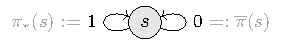
\includegraphics[width=0.35\linewidth]{figures/mdp.pdf}
        \caption{MDP}
        \label{fig: experiment smallest MDP for iv vs fv}
    \end{subfigure}%
    \\
    \vspace{0.5cm}
    % --- Subfigure 1: Streamlines ---
    \begin{subfigure}[b]{0.48\textwidth}
        % \begin{tikzpicture}
        %     \begin{axis}[
        %         width=\linewidth,
        %         % title={Initial-visit solutions},
        %         xlabel={$q(s, \pi_*(s))$},
        %         ylabel={$q(s, \overline \pi(s))$},
        %         tick label style={font=\small},
        %         label style={font=\small},
        %         xmin=0, xmax=5,
        %         ymin=-0.5, ymax=4.5,
        %         % grid=off,
        %         axis equal image,
        %         unbounded coords=jump, % This handles the NaN values in your CSV
        %         xtick={1, 2,4},
        %         % xticklabels={1, $\frac{1}{1-\gamma}$, 4},
        %         ytick={0, 1,4}
        %     ]

        %         \addplot [black, thin, dotted, domain=-0.5:5, samples=2] {x};
                
        %         % 1. Plot the streamlines from CSV
        %         \addplot[mygrey, thin, forget plot] table [col sep=comma, x index=0, y index=1] {figures/streamlines-iv.csv};

        %         % 2. Plot the simulation trajectory
        %         \addplot[CambridgeCoreBlue, thick] table [col sep=comma, x index=0, y index=1] {figures/simulation-iv-above.csv};

        %         \addplot[CambridgeCoreBlue, thick] table [col sep=comma, x index=0, y index=1] {figures/simulation-iv-below.csv};
                
        %         % 3. Mark Attractors (x1 and x2 based on your gamma=0.5)
        %         \node[label={right:$q_{\pi_*}$}, circle, fill, inner sep=1.5pt] at (axis cs:2, 1) {};
                
        %         \node[label={right:$q_{\overline \pi}$}, circle, fill, inner sep=1.5pt] at (axis cs:1,0) {};
                
        %         % 4. Start Points with Labels
        %         % Point A: Using your x0 = [3.75, 4]
        %         \node[label={left:$q$}, circle, fill, inner sep=1.5pt, CambridgeCoreBlue] at (axis cs:3.75, 4) {};
                
        %         % Point B: Placeholder (Update coordinates as needed)
        %         \node[label={below:$q'$}, circle, fill, inner sep=1.5pt, CambridgeCoreBlue] at (axis cs:4, 3.75) {};
        %     \end{axis}
        % \end{tikzpicture}
        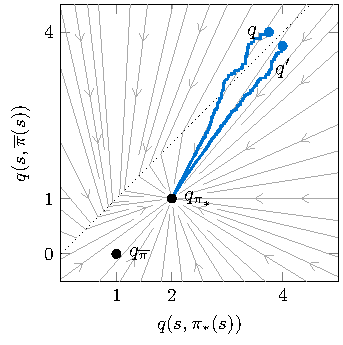
\includegraphics[width=0.8\linewidth]{figures/iv-sol.pdf}
        \caption{Initial-visit solutions}
        \label{fig: iv versus fv simulations IV}
    \end{subfigure}
    \hfill
    % --- Subfigure 2: Placeholder or Second Simulation ---
    \begin{subfigure}[b]{0.48\textwidth}
        % \begin{tikzpicture}
        %     \begin{axis}[
        %         width=\linewidth,
        %         % title={First-visit solutions},
        %         xlabel={$q(s, \pi_*(s))$},
        %         ylabel={$q(s, \overline \pi(s))$},
        %         tick label style={font=\small},
        %         label style={font=\small},
        %         xmin=0, xmax=5,
        %         ymin=-0.5, ymax=4.5,
        %         % grid=off,
        %         axis equal image,
        %         unbounded coords=jump, % This handles the NaN values in your CSV
        %         xtick={1, 2,4},
        %         % xticklabels={1, $\frac{1}{1-\gamma}$, 4},
        %         ytick={0, 1,4}
        %     ]

        %         \addplot [black, thin, dotted, domain=-0.5:5, samples=2] {x};
                
        %         % 1. Plot the streamlines from CSV
        %         \addplot[mygrey, thin, forget plot] table [col sep=comma, x index=0, y index=1] {figures/streamlines-fv.csv};

        %         % 2. Plot the simulation trajectory
        %         \addplot[CambridgeCoreBlue, thick] table [col sep=comma, x index=0, y index=1] {figures/simulation-fv-above.csv};

        %         \addplot[CambridgeCoreBlue, thick] table [col sep=comma, x index=0, y index=1] {figures/simulation-fv-below.csv};
                
        %         % 3. Mark Attractors (x1 and x2 based on your gamma=0.5)
        %         \node[label={right:$q_{\pi_*}$}, circle, fill, inner sep=1.5pt] at (axis cs:2, 1) {};
                
        %         \node[label={right:$q_{\overline \pi}$}, circle, fill, inner sep=1.5pt] at (axis cs:1,0) {};
                
        %         % 4. Start Points with Labels
        %         % Point A: Using your x0 = [3.75, 4]
        %         \node[label={left:$q$}, circle, fill, inner sep=1.5pt, CambridgeCoreBlue] at (axis cs:3.75, 4) {};
                
        %         % Point B: Placeholder (Update coordinates as needed)
        %         \node[label={below:$q'$}, circle, fill, inner sep=1.5pt, CambridgeCoreBlue] at (axis cs:4, 3.75) {};
        %     \end{axis}
        % \end{tikzpicture}
        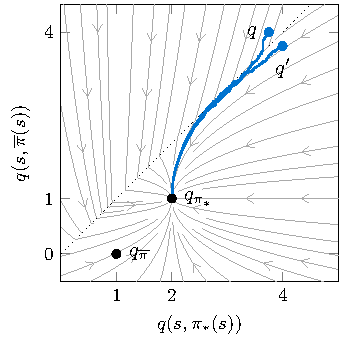
\includegraphics[width=0.8\linewidth]{figures/fv-sol.pdf}
        \caption{First-visit solutions}
        \label{fig: iv versus fv simulations FV}
    \end{subfigure}
    \caption{By avoiding sliding modes, initial-visit solutions sometimes converge to the optimal policy $\best{\pi}$ faster than first-visit solutions despite fewer updates and smaller effective learning rates. The blue lines are MC-O-PI solutions starting in $q$ or $q'$, whereas the grey lines indicate the mean-field flow.}
    \label{fig: iv versus fv simulations}
\end{figure}



%%%%%%%%%%%%%%%%%%%%%%%%%%%%%%%%%%%%%%%%%%%%%%%%%%%%%%%%%%%%%%%%%%%
%%%%%%%%%%%%%%%%%%%%%%%%%%%%%%%%%%%%%%%%%%%%%%%%%%%%%%%%%%%%%%%%%%%
%\subsection{Guaranteeing convergence with non-uniform updates}

% The practical takeaway from this paper is simple: if MC-O-PI seems trapped in a suboptimal limit set (on a boundary or in a cycle), 
% then using initial-visit updates
% with uniform sampling distributions over the actions in each state
% guarantees that the algorithm eventually converges to the optimal policy and its action values
% while avoiding slow sliding modes.

% In order to turn non-uniform update distributions into uniform effective updates, \cite{Tsitsiklis2002OnIteration} suggests making the learning rates inversely proportional to the update distribution.
% In a model-free setting, this strategy only applies if the update distributions are generated with the initial-visit method.
% This is because the first-visit method causes the update distributions to depend on the transition dynamics induced by the currently greedy policy on the MDP.
% Since the greedy policy changes at every step and the structure of the MDP is unknown,
% we must assume that first-visit update distributions change at every step.
% Cancelling out these changing, non-uniform distributions thus requires knowing the induced transition dynamics, which are unpredictable if the MDP is unknown.

% Nonetheless, consider non-uniform, initial-visit update distributions $(\mu_k)_{k \ge 0}$, which essentially equal the sampling distributions $(\sigma_k)_{k \ge 0}$.
% For any scalar sequence $(\lambda_k)_{k \ge 0}$ that satisfies the Robbins--Monro conditions,
% if the $k^\nth$ episode starts in $(s_0, a_0)$, then setting
% \[
%     \alpha_k = \frac{\lambda_k}{\sigma_k(s_0, a_0)} , 
% \]
% guarantees that the effective learning rates in MC-O-PI's difference inclusion are uniform because $\alpha_k \, \mu_k(s_0, a_0) = \lambda_k$.
% However, this approach is impractical because it requires knowing the sampling probability for each state-action pair at every step,
% or, if these probabilities are constant over time, tracking the number of updates of each state-action pair \citep[p.~66]{Tsitsiklis2002OnIteration}.


% Tsitsiklis notes that MC-O-PI's asymptotic behaviour depends on the asymptotic behaviour of the effective learning rates $(\lrate_k \update_k)$, not on either component alone.
% For instance, if the update distributions are non-uniform but constant, say $\update_k = \update$ for all $k$, and the learning rates take the form $\lrate_k(s,a) = 1/n_k(s,a)$, where $n_k(s,a)$ denotes the number of updates of $(s,a)$ in the first $k$ steps,
% then $\lrate_k \update_k$ converges to $1/k$ because for each state-action pair $n_k(s,a)$ tends to $k \update(s,a)$. As a result, updates are eventually uniform. So \autoref{thm: convergence mcopi uniform} still applies.


% In contrast, we showed that global convergence only requires uniform updates over all actions in each state.
% Using the decomposition
% \[
% \sigma_k(s,a) = \sigma^{\sset}_k(s) \, \sigma^{\aset}_k(a \mid s)
% \]
% where $\sigma^{\sset}$ represents the sampling distribution over the state space,
% and $\sigma^{\aset}$ is the distribution over the action space of each state,
% it is thus sufficient to choose learning rates as
% \[
%     \alpha_k = \frac{\lambda_k}{\sigma^{\aset}_k(a_0 \mid s_0)}.
% \]
% This is more practical because it only assumes knowing the sampling probability of the initial action $a_0$ relative to the other actions of the initial state $s_0$, rather than all other state-action pairs.
% In other words, we can obtain global convergence 
% by turning non-uniform update distributions 
% into uniform effective updates even if the initial state is sampled from an unknown distribution, provided the distribution of the initial action in that state is known. This occurs in practice, for instance, when selecting the initial action using an $\varepsilon$-greedy strategy.


% A concrete example of a non-uniform update distribution arises when biasing updates towards the greedy actions to \textit{exploit} the policy that is currently believed to be optimal.
% However, by unevenly updating actions, this approach causes non-greedy actions to evolve very slowly and potentially leads to the sliding modes depicted in \autoref{fig: iv versus fv simulations}.
% Therefore, if we additionally scale down the learning rates for the greedy actions in proportion to their increased update probability (so that the product $\alpha_k(s,a)\,\mu_k(s,a)$ does not depend on $a$),
% then updates are effectively uniform over the actions of each state, and global convergence is guaranteed.
% Notably, this adjustment does not violate the comparability property (\autoref{asp: additional conditions on learning rate}) required by \autoref{thm: convergence mcopi uniform}. Although learning rates may fail global comparability across the entire process, the proof only uses the comparability property between transitions, which matches the intervals in which the greedy actions remain the same.
% An additional benefit of making the learning rates inversely proportional to the update distribution is that this reduces the variance of the estimate $q_k$ for greedy actions, which means the solution remains closer to the well-behaved mean-field solution along that dimension.
% On the other hand, the larger learning rates for non-greedy actions compensate for their infrequent updates but at the cost of slightly increased variance.
% Ultimately, this learning rate adjustment 
% % removes the convergence difficulties seen with purely greedy updates (such as slow learning for non-greedy actions, or sliding modes), keeps all trajectories well-behaved, and 
% ensures that all action values converge at similar rates along approximately straight trajectories towards the optimum.


% %%%%%%%%%%%%%%%%%%%%%%%%%%%%%%%%%%%%%%%%%%%%%%%%%%%%%%%%%%%%%%%%%%%
% %%%%%%%%%%%%%%%%%%%%%%%%%%%%%%%%%%%%%%%%%%%%%%%%%%%%%%%%%%%%%%%%%%%
% \subsection{Importance of noise}
% \label{sec: discussion noise}


% general comment to anybody studying
% switching linear system

% stochastic difference equation

% proof is not an iff

% stochastic solutions can lock into the region of a policy thanks to noise even when the mean-field




%%%%%%%%%%%%%%%%%%%%%%%%%%%%%%%%%%%%%%%%%%%%%%%%%%%%%%%%%%%%%%%%%%%
%%%%%%%%%%%%%%%%%%%%%%%%%%%%%%%%%%%%%%%%%%%%%%%%%%%%%%%%%%%%%%%%%%%
\subsection{Mean-field analysis with temporal difference updates}
\label{sec: discussion temporal difference}

The gap estimate uses conditional drift and variance bounds, while the favorable-update construction uses a bounded number of requests regardless of the waiting time. An analogous approach to temporal-difference updates would additionally need a policy-improvement mechanism and a favorable-update construction compatible with targets that change with the current estimate. The present theorem does not establish those properties.
The additional difficulty would be to understand how the estimate $q$ and the simulation depth $n$ affect the target $T_{\pi}^n q$, where $\pi \in P(q)$. Here $T_\pi$ is the action-value Bellman operator,
\[
(T_\pi q)(s,a)=\mathbb E_p\!\left[r_0+\gamma q(s_1,\pi(s_1))\mid s_0=s,a_0=a\right],
\]
and the superscript $n$ denotes repeated composition.


%%%%%%%%%%%%%%%%%%%%%%%%%%%%%%%%%%%%%%%%%%%%%%%%%%%%%%%%%%%%%%%%%%%
%%%%%%%%%%%%%%%%%%%%%%%%%%%%%%%%%%%%%%%%%%%%%%%%%%%%%%%%%%%%%%%%%%%
\subsection{MC-O-PI with function approximation}
\label{sec: discussion function approximation}

\autoref{thm: convergence mcopi uniform} applies specifically to \textit{tabular} MC-O-PI, where the estimate $q_k$ can be stored exactly.
In practical applications, however, the estimate is approximated, for instance using a neural network.
In this setting, the error between the observed return and the current estimate is then used to update the parameters of the approximation.
% for instance using gradient descent.

Extending the theorem would require quantitative control of accumulated approximation errors and a replacement for the favorable-update argument for individual state-action pairs. Representational richness alone does not provide either property. Perturbation analyses such as \citet[Section~4.3.3]{Bertsekas1996Neuro-DynamicProgramming} and \citet[Section~5.2]{Kushner2003StochasticApplications} suggest possible tools, but their applicability to this extension remains to be established.
%Furthermore, integrating a normalisation trick as in \autoref{sec: normalisation trick} into Monte Carlo Tree Search might accelerate AlphaZero's or MuZero's learning process by mitigating slow sliding modes.

% Finally, \citet{Wagner2013OptimisticResult} shows that policy gradient methods
% % which underlie recent breakthroughs in natural language processing and robotics \citep{Schulman2017ProximalAlgorithms}, 
% can be interpreted as optimistic policy iteration algorithms with function approximation. Extending our results to this setting might
% thus improve the efficiency and performance of these essential methods.


Finally, recent breakthroughs in natural language processing and robotics~\citep{Schulman2017ProximalAlgorithms} rely on policy gradient methods.
\citet{Wagner2013OptimisticResult} shows that some of these methods can be interpreted as optimistic policy iteration algorithms with function approximation.
Extending our results to this setting might thus improve the efficiency and performance of these essential methods.


% \textcolor{red}{still necessary?}

% Applying the method of \autoref{sec: results} when update distributions are uniform over all state-action pairs 
% reveals a Lyapunov interpretation of Tsitsiklis' framework.
% Namely, consider the potential function that measures the one-sided Bellman residual
% \begin{align}
%     \tilde V(q) = \frac{1}{2} \|(q-\B q)_+\|_2^2 .
% \end{align}
% Its gradient is
% \begin{align}
%     \nabla \tilde V (q) = (I - \discount P_\pi )^\top (q-\B q)_+
% \end{align}
% where $\pi$ is any deterministic policy that is greedy with respect to $q$.
% Computing the inner product with the mean-field update of MC-O-PI yields
% \begin{align*}
%     \langle \nabla \tilde V(q) , q_\pi - q \rangle
%     &= \langle (I - \discount P_\pi )^\top (q-\B q)_+ , (I - \discount P_\pi )^{-1} (\B q - q) \rangle
%     \\
%     &= \langle (q-\B q)_+ , (\B q - q) \rangle
%     \\
%     &= - \|(q - \B q)_+\|_2^2
%     \\
%     &= - 2 \tilde V(q)
% \end{align*}
% Thus, when updates are uniform over all state-action pairs, the mean-field update $(q_\pi - q)$ is a strict descent direction for the potential $\tilde V$.
% This geometric insight corresponds to the decrease in inequality \eqref{eq: q-Bq decreases} that is essential to Tsitsiklis' proof.
% % That proof thus exploits the tension between the fact that every limit point is upper and lower bounded by the best and worst action values of the corresponding greedy policies (\autoref{thm: bounded limit sets})
% % and that such point has a strictly positive one-sided Bellman residual (\autoref{thm: bellman residual has positive component}).
% The proof in \autoref{sec: results} builds on this insight. 
% Unlike Tsitsiklis' method, our proof does not rely on the commutativity of the transition matrix $P_\pi$ and the update distribution $\mu$. The trade-off is that we must instead constrain the variation of the update distribution to ensure that the local descent property is preserved.
% Yet, as discussed earlier, we expect that this conditions can be relaxed.

% We note that Tsitsiklis extends his proof to optimistic policy iteration with temporal difference returns, i.e. where the target $q_\pi$ is replaced by a geometrically weighted sum of multi-step returns (TD($\lambda$)).
% This introduces an additional error term in the descent inequality \eqref{eq: q-Bq decreases}. Given the structural similarities, we conjecture that the framework of \autoref{sec: results} can be similarly extended. Future work could apply our method to TD-O-PI, where an analogous summable error term would likely appear in the critical inequality \eqref{eq: V goes to infinity}, potentially establishing convergence for TD control under our broader class of update distributions.


% Tsitsiklis proof also works with temporal difference optimistic policy iteration
% $n$-step TD-O-PI is when updates are
% \begin{align}
%     q_{k+1} \in 
%     \{
%     q+k + \lrate_k \update_k (\B_\pi^n q_k - q_k + w_k)
%     \}
% \end{align}
% with the appropriate definition of stochastic perturbations.
% so $n=1$ is q learning whereas $n=\infty$ is MC-O-PI

% not sure whether the argument is exactly symmetrical ...
% the argument in \autoref{sec: results} is symmetrical. All that matters is that $\bqar q \neq \B \bar q$. either focus on state-action pairs where $[\bar q(s,a) - \B \bar q](s,a)>0$ and then use the definition of $g_\pi$ and $V$ as above. or focus on states where $[\bar q(s,a) - \B \bar q](s,a) < 0$ and then use the definition of $g_\pi \coloneqq \mu^{-1} (I - \discount P_\pi^\top)(\B \bar q - q)_+$ and $V(q) \coloneqq \min_\pi \langle g_\pi, q - \bar q \rangle$ and show that $q_k \to \bar q$ drives V to $- \infty$.


%%%%%%%%%%%%%%%%%%%%%%%%%%%%%%%%%%%%%%%%%%%%%%%%%%%%%%%%%%%%%%%%%%%
%%%%%%%%%%%%%%%%%%%%%%%%%%%%%%%%%%%%%%%%%%%%%%%%%%%%%%%%%%%%%%%%%%%
\subsection{Sampling, learning rates and policy ties}
\label{sec: relaxing conditions}
The theorem requires infinite accumulated learning at every state, $\sum_k\alpha_k\sigma_k(s)=\infty$, but no positive lower sampling bound and no bound on the waiting time between updates. This distinction matters for a global learning-rate sequence: infinitely many visits can carry only finite total weight. The deterministic argument needs only the divergent effective weights and coefficients in $[0,1]$; square summability is used to control stochastic errors.

Inertia in greedy policy selection, as in \eqref{eq:greedy-pol-tie-breaking}, is convenient for the proof. Fixed action priorities give the same convergence conclusion, provided the priorities are used consistently from initialization. The only change is the local retention argument: raising the reference estimate, lowering a competitor, or leaving a state's table unchanged cannot introduce a higher-priority maximizer. Thus unfinished states retain their reference actions during the favorable-update construction, and the rest of the proof is unchanged. Fresh random tie-breaking would require a different retention argument and is not included in the theorem as stated.

The learning-rate condition bounds future increases by a fixed factor; it allows infinitely many increases and imposes no comparability lower bound on future steps. It is used twice: earlier favorable updates must be large enough relative to the eventual completion step, and future noise must be controlled relative to the gap created at completion. Whether this regularity can be removed from the stochastic theorem remains open here. Its role in the proof does not establish its necessity for convergence.

\section{Conclusion}


%\textcolor{red}{mention that our result make more sense / uniform over all state-action pairs automatically forces more frequent updates to states with more actions, which does not really make sense}


 % 1. Finding = what did we find
We established that the mean-field dynamics of Monte Carlo optimistic policy iteration drive trajectories toward monotonically improving policies when updates are uniform over all actions in each state. 
We then proved that the stochastic perturbations cannot systematically counteract this improvement,
and consequently that MC-O-PI converges to the optimal action values when updates are uniform.


% Consequence of the result
This result extends existing convergence guarantees to more practical settings. Unlike previous proofs that required uniform updates across all state-action pairs, our analysis allows different states to be updated at different frequencies.
This relaxation makes the algorithm applicable to large-scale problems where uniform sampling over the joint state-action space is not feasible.
The guarantee allows such state-dependent sampling under the stated cumulative-learning, return-moment, tie-breaking and learning-rate conditions.
% Instead, learning can prioritise different states at different times by sampling the initial states of episodes accordingly.
% As long as every state is sampled infinitely often and all actions of each state are updated equally frequently, MC-O-PI eventually converges to the optimal policy and action values. 


% consequence of the method
We extended the lock-in strategy of the combined stability-ODE method to accommodate the discontinuous dynamics of MC-O-PI.
This mean-field approach provided a more intuitive explanation for the convergence mechanism than previous proofs that directly tackled the stochastic process.
More importantly, it opens up new possibilities, beyond contraction-based analysis, to study the convergence of optimistic policy iteration algorithms.


% perspectives
We see three principal directions for future work:
(1) determine whether the remaining step-size regularity can be weakened further,
% (2) find whether the optimal action values remain globally stable for mean-field solutions of MC-O-PI when updates are non-uniform,
(2) apply this new method to study the convergence of optimistic policy iteration algorithms that rely on temporal difference evaluation,
and (3) generalise our result when value estimates are stored approximately.



% Afterwards, there would be insane potential to generalise the results to the function approximation case.
% \textcolor{red}{because ...}

% Generalizing our results to function approximation opens substantial opportunities.
% \citet{Wagner2013OptimisticResult} show that optimistic policy iteration with approximation is closely connected to policy gradient methods.
% These methods underpin many of the most impactful advances in artificial intelligence, including large language models and robotics.
% Extending our guarantees to this setting could lead to faster learning and stronger performance guarantees, enabling the reliable computation of higher-quality policies in complex environments.


% relaxing constraints that are not necessary to preserve the mean-field improvement property,
% % (see section \ref{sec: relaxing conditions}),
% and extending the analytical framework to temporal difference methods.
% % (see section \ref{sec: discussion tsitsiklis link}).


% can use the same approach when estimates are biased, but bias decreases over time => multi-step TD


% PERSPECTIVES = generalise
% Feedback from Silver
% discussion that connects the algorithms to real world impact
% - discussion of the exploration-exploitation trade-off that is so fundamental to RL (beyond introducing GLIE and an aside in 6.2.6)
% - some discussion of function approximation (at least to say that the majority of practical applications would need to also bring in function approximation), 
% - scalable algorithms that build upon Monte-Carlo learning (e.g. Monte-Carlo tree search)
% - some additional axes of reinforcement learning, such as on-policy/off-policy, model-free/model-based, value-based/actor-critic/policy-based -
% would any of the insights in this thesis generalize along any of these axes?



\clearpage


\appendix
\section*{Appendix}
\label{sec: Appendix}

\paragraph{Proof of \autoref{thm: properties of noise}}

Fix a time $k\ge 0$, a state $s \in \mathcal S$ and an action $a \in \mathcal A(s)$.

By definition,
\begin{align}
\label{eq: noise def in appendix proof}
w_k(s,a) = u_k(s,a) v_k(s,a) + \big( u_k(s,a)-\mu_k(s,a) \big) \big( q_{\pi_k}(s,a) - q_k(s,a) \big).
\end{align}
By the return-moment assumption \eqref{eq: return moments},
and $u_k(s,a) v_k(s,a) = 0$ on $\{u_k(s,a)=0\}$,
it follows that
\begin{align}
\label{eq: unbiased noise p1}
\mathbb E[ u_k(s,a) v_k(s,a) \mid \mathcal F_k']
=
\mathbb E \big[
    \mathbf 1_{\{u_k(s,a)=1\}} \mathbb E[ v_{k}(s,a) \mid \mathcal F_k', u_k(s,a)=1]
    \mid \mathcal F_k' \big]
= 0 .
\end{align}
Also, $\mathbb E[u_k(s,a) \mid \mathcal F_k'] = \mu_k(s,a)$, and $\mu_k$ and $q_{\pi_k}-q_k$ are $\mathcal F_k'$-measurable. Hence,
\begin{multline}
\label{eq: unbiased noise p2}
\mathbb E \!\left[
\bigl( u_k(s,a)-\mu_k(s,a) \bigr) \bigl( q_{\pi_k}(s,a)-q_k(s,a) \bigr)
\mid \mathcal F_k'
\right]
\\
=
\big( q_{\pi_k}(s,a)-q_k(s,a) \big)
\big( \mathbb E\!\left[ u_k(s,a) \mid \mathcal F_k'
\right]
-\mu_k(s,a) \big)
=
0 .
\end{multline}
Summing \eqref{eq: unbiased noise p1} and \eqref{eq: unbiased noise p2} yields $\mathbb E[w_k(s,a) \mid \mathcal F_k'] = 0$.
This proves \eqref{eq: muw_mds}.

Finally, since $u_k^2(s,a) \le 1$ and $(u_k(s,a) - \mu_k(s,a))^2 \le 1$,
using $(x+y)^2 \le 2 x^2 + 2 y^2$ on \eqref{eq: noise def in appendix proof} yields
\begin{align*}
w_k^2(s,a)
&\le 2 v_k^2(s,a) + 2 (q_{\pi_k}(s,a)-q_k(s,a) )^2
\\
&\le 2 v_k^2(s,a) + 2 ( 2 q_{\pi_k}^2(s,a) + 2 q_k^2(s,a) ) .
\end{align*}
Since all action-values are bounded,
there exists a constant $c_\polset < \infty$ such that $\|q_\pi\|^2 \leq c_\polset$ for every policy $\pi \in \polset$. As a result,
\begin{align*}
\mathbb E \!\big[ w_{k}^2(s,a) \mid \mathcal F'_k \big]
&\le
2 c_v + 2 \, \mathbb E \!\left[ ( q_{\pi_k}(s,a)-q_k(s,a) )^2 \mid \mathcal F'_k \right]
\\
&\le
2 c_v + 4 c_\polset + 4 \|q_k\|^2
\end{align*}
So \eqref{eq: muw_second_moment} holds for example with $c_w := \max \{ 2 c_v + 4 c_\polset, 4\}$.
\hfill \BlackBox

\paragraph{Fixed-target averages.}
\label{app: fixed target averages}
The comparison argument for boundedness and the convergence of a constant-target block both use the following consequence of the supermartingale convergence theorem~\citep[Proposition~4.2]{Bertsekas1996Neuro-DynamicProgramming}: if a nonnegative process has conditional expected increments bounded above by a negative term plus a summable error, then it converges and the negative terms have finite sum.

Fix a deterministic restart $r$, a policy $\pi\in\mathcal P$ and a state-action pair $(s,a)$.
Starting from $x_r=q_r(s,a)$, consider the average with fixed target $q_\pi(s,a)$,
\[
x_{k+1}=x_k+\alpha_k u_k(s,a)\big(q_\pi(s,a)+v_k(s,a)-x_k\big).
\]
The initial squared error is integrable: finite-time estimates have finite second moments by induction in \eqref{eq: update q with chi} and \eqref{eq: return moments}.
Since $u_k(s,a)$ is an indicator with conditional mean $\sigma_k(s,a)$, the return moments and $0<\alpha_k\le1$ give
\[
\mathbb E\!\left[(x_{k+1}-q_\pi(s,a))^2\mid\mathcal F'_k\right]
\le (1-\alpha_k\sigma_k(s,a))(x_k-q_\pi(s,a))^2+c_v\alpha_k^2.
\]
The cited theorem shows that $(x_k-q_\pi(s,a))^2$ converges and that
\[
\sum_{k=r}^{\infty}\alpha_k\sigma_k(s,a)(x_k-q_\pi(s,a))^2<\infty
\quad\text{almost surely}.
\]
Its limit must be zero, since \eqref{eq: cumulative learning} makes the sum of the weights infinite.
These assertions hold simultaneously for every deterministic integer $r$, every policy and every state-action pair: take the intersection of their countably many probability-one events. We may therefore choose a restart and a target separately on each resulting path, without conditioning on their future-dependent values.

\paragraph{Proof of \autoref{thm: bounded limit sets}}
Let $(q_k)$ and $(\pi_k)$ be an MC-O-PI solution satisfying \autoref{asp: standing}, and work on the probability-one event just obtained. Since the policy set is finite, there is a finite index $r$ after which only policies in $\polset_\infty$ appear.
Thus for all $k\ge r$ and every pair $(s,a)$,
\[
\min_{\pi\in\polset_\infty}q_\pi(s,a)
\le q_{\pi_k}(s,a)
\le\max_{\pi\in\polset_\infty}q_\pi(s,a).
\]
Start $x_r=y_r=q_r(s,a)$ and use the same sampled updates and return noise, with the two fixed targets:
\begin{align*}
x_{k+1}&=x_k+\alpha_k u_k(s,a)
\left(\min_{\pi\in\polset_\infty}q_\pi(s,a)+v_k(s,a)-x_k\right),\\
y_{k+1}&=y_k+\alpha_k u_k(s,a)
\left(\max_{\pi\in\polset_\infty}q_\pi(s,a)+v_k(s,a)-y_k\right).
\end{align*}
Because $0\le\alpha_k u_k(s,a)\le1$, induction gives $x_k\le q_k(s,a)\le y_k$ for every $k\ge r$.
Each comparison target is one of the finitely many values covered by the preceding fixed-target calculation. Consequently,
\begin{align*}
\liminf_{k\to\infty}q_k(s,a)&\ge\min_{\pi\in\polset_\infty}q_\pi(s,a),\\
\limsup_{k\to\infty}q_k(s,a)&\le\max_{\pi\in\polset_\infty}q_\pi(s,a).
\end{align*}
This proves convergence to the stated bounded set. In particular, the estimates are bounded along almost every path. If the actual target is eventually constant, the estimate itself is one of the fixed-target averages above, which also justifies its use in \autoref{thm: suboptimal blocks finite}.
\hfill\BlackBox

\paragraph{Proof of \autoref{thm: convergence deterministic mcopi}}
Let $(q_k)$ be a solution of the mean-field dynamics \eqref{eq: deterministic mcopi} under the stated assumptions, with policies $(\pi_k)$ and transition times $(t_n)$.
\autoref{thm: improving policies} shows that their action-value functions are nondecreasing and change only by improvements. Since there are finitely many deterministic policies, the target is constant from some finite transition time $t_n$ onwards.
For every pair $(s,a)$ and every $k\ge t_n$, unrolling the deterministic recursion gives
\[
q_k(s,a)-q_{\pi_{t_n}}(s,a)
=\big(q_{t_n}(s,a)-q_{\pi_{t_n}}(s,a)\big)
\prod_{j=t_n}^{k-1}(1-\alpha_j\mu_j(s,a)).
\]
The product tends to zero because $\sum_j\alpha_j\mu_j(s,a)=\infty$.
A policy appearing infinitely often in the remaining sequence has action values $q_{\pi_{t_n}}$; passing its greedy inequalities to the limit shows that it is greedy for its own action values, hence optimal. Therefore $q_{\pi_{t_n}}=q_{\pi_*}$ and $q_k\to q_{\pi_*}$.
\hfill\BlackBox

\paragraph{Proof of \autoref{lem:measure}}
At a requested update of state $s$, let $p_k(s)$ be the conditional probability of the favorable action and return event, given $\mathcal F'_k$ and that state $s$ is selected. By \eqref{eq:localprob}, $p_k(s)\ge p_0$ on positive-probability selections. Values at zero-probability selections may be assigned arbitrarily.

Starting with $L_t=1$, multiply $L_k$ by the indicator that the requested update succeeds, divided by $p_k(s)$. At iterations without a request, use factor one. Each factor has conditional mean one given the current history and selected state. Thus
\[
\mathbb E[L_{k+1}\mid\mathcal F'_k]=L_k.
\]
This is the martingale property: knowing the present history does not change the expected future weight. At most $|\mathcal S\times\mathcal A|N$ factors differ from one, so
\[
0\le L_k\le p_0^{-|\mathcal S\times\mathcal A|N}.
\]
The weight is eventually constant on each path, even though there is no bound on the times of the requested updates. Denote its limit by $L_\infty$. The common deterministic bound permits passing expectations through the limit. Indeed, for every $\varepsilon>0$,
\[
\mathbb E|L_k-L_\infty|
\le\varepsilon+2p_0^{-|\mathcal S\times\mathcal A|N}
\mathbb P(|L_k-L_\infty|>\varepsilon),
\]
and the probability tends to zero. Letting $\varepsilon$ decrease to zero gives convergence in mean.
For every event $A$ known from $\mathcal F'_t$, the martingale identity consequently gives
\[
\mathbb E[\mathbf1_A L_\infty]=\mathbb P(A).
\]
These identities mean that $\mathbb E[L_\infty\mid\mathcal F'_t]=1$: a conditional expectation is the quantity determined by the conditioning history that reproduces the original average on each event known from that history. The same argument at later histories gives $\mathbb E[L_\infty\mid\mathcal F'_k]=L_k$.

Define the auxiliary law by
\[
\widehat{\mathbb P}(E)=\mathbb E[L_\infty\mathbf1_E].
\]
It assigns more weight to runs with successful seed updates. A failed request makes $L_\infty=0$, so all requests succeed under this law. An event of original probability zero still has probability zero after reweighting.
For a random start $t$, use weight one before $t$, on $\{t=\infty\}$ and when $t\ge\zeta_r$, and combine the fixed-start constructions on $\{t=j\}$ over integers $j$. Each of these events is known at time $j$, so the same conditional argument applies.

It remains to check that future requests do not bias updates at completed states. If a bounded random variable $Y$ is determined by the next history $\mathcal F'_{k+1}$, then on $\{L_k>0\}$,
\begin{equation}
\label{eq: weighted conditional law}
\widehat{\mathbb E}[Y\mid\mathcal F'_k]
=\frac{\mathbb E[L_\infty Y\mid\mathcal F'_k]}{L_k}
=\frac{\mathbb E[L_{k+1}Y\mid\mathcal F'_k]}{L_k}.
\end{equation}
For the first equality, test the proposed conditional expectation against any event $A$ known at $k$. The definition of the weighted law and $\mathbb E[L_\infty\mid\mathcal F'_k]=L_k$ give
\[
\widehat{\mathbb E}\!\left[\mathbf1_A
\frac{\mathbb E[L_\infty Y\mid\mathcal F'_k]}{L_k}\right]
=\mathbb E[\mathbf1_A L_\infty Y]
=\widehat{\mathbb E}[\mathbf1_A Y].
\]
The fraction is defined as zero where $L_k=0$; nonnegativity and the conditional-mean identity imply that those histories have auxiliary probability zero. The second equality in \eqref{eq: weighted conditional law} uses $\mathbb E[L_\infty\mid\mathcal F'_{k+1}]=L_{k+1}$, so all later request factors average out, even when the later requests depend on the present return.

The current factor $L_{k+1}/L_k$ has conditional mean one given the history and selected state. Applying \eqref{eq: weighted conditional law} to the indicator that a particular state is selected therefore preserves state-selection probabilities. If that state is complete, the current factor is exactly one. Conditioning further on its selection consequently leaves the action and return law unchanged. The same holds after the construction stops. The algorithmic identities and the inertia rule also remain valid, since originally null events remain null.
Finally,
\[
\widehat{\mathbb P}(E\mid\mathcal F'_t)
=\mathbb E[L_\infty\mathbf1_E\mid\mathcal F'_t]
\le p_0^{-|\mathcal S\times\mathcal A|N}\mathbb P(E\mid\mathcal F'_t),
\]
which is \eqref{eq:transfer}. This reweighting is only a proof device; the algorithm continues to sample its original returns.
\hfill\BlackBox

\paragraph{The martingale maximal inequality used in \autoref{lem:barrier}}
\label{app: martingale bound}
For a sum $M_n$ of increments with zero conditional mean, distinct increments have zero expected product. Its second moment is therefore the sum of their second moments. To bound its largest deviation, first fix a finite horizon $N$ and let $\theta$ be the first index at which $|M_\theta|\ge z$, where $M$ starts from zero and $z>0$ is known at the restart time.
On $\{\theta=j\}$ the later increment $M_N-M_j$ has conditional mean zero. Expanding the square gives
\[
\mathbb E[\mathbf1_{\{\theta=j\}}M_N^2]
\ge \mathbb E[\mathbf1_{\{\theta=j\}}M_j^2]
\ge z^2\mathbb P(\theta=j).
\]
Summing over $j\le N$ bounds the crossing probability by $\mathbb E[M_N^2]/z^2$.
Multiplying throughout by indicators of events known at the restart gives the conditional version. Stopping a sum preserves its zero conditional means, because the decision to retain an increment is made before drawing it. Apply the finite-horizon bound to the stopped sum and then increase $N$. For an infinite horizon, approach a possibly unattained threshold from below. For thresholds and variance bounds determined by the restart history, the same argument is applied conditionally; one may first restrict them to bounded ranges and then increase those ranges. Random restart times are handled on their individual finite-time events. These steps justify the conditional maximal estimates in the growth and lock-in argument without a bound on waiting times.



% Acknowledgements and Disclosure of Funding should go at the end, before appendices and references

\acks{This research was supported by the MathWorks Studentship.}

% Manual newpage inserted to improve layout of sample file - not
% needed in general before appendices/bibliography.

% \newpage




% \section{}
% \label{app:theorem}

% % Note: in this sample, the section number is hard-coded in. Following
% % proper LaTeX conventions, it should properly be coded as a reference:

% %In this appendix we prove the following theorem from
% %Section~\ref{sec:textree-generalization}:

% In this appendix we prove the following theorem from
% Section~6.2:

% \noindent
% {\bf Theorem} {\it Let $u,v,w$ be discrete variables such that $v, w$ do
% not co-occur with $u$ (i.e., $u\neq0\;\Rightarrow \;v=w=0$ in a given
% dataset $\dataset$). Let $N_{v0},N_{w0}$ be the number of data points for
% which $v=0, w=0$ respectively, and let $I_{uv},I_{uw}$ be the
% respective empirical mutual information values based on the sample
% $\dataset$. Then
% \[
% 	N_{v0} \;>\; N_{w0}\;\;\Rightarrow\;\;I_{uv} \;\leq\;I_{uw}
% \]
% with equality only if $u$ is identically 0.} 
% \hfill\BlackBox

% \noindent
% {\bf Proof}. We use the notation:
% \[
% P_v(i) \;=\;\frac{N_v^i}{N},\;\;\;i \neq 0;\;\;\;
% P_{v0}\;\equiv\;P_v(0)\; = \;1 - \sum_{i\neq 0}P_v(i).
% \]
% These values represent the (empirical) probabilities of $v$
% taking value $i\neq 0$ and 0 respectively.  Entropies will be denoted
% by $H$. We aim to show that $\fracpartial{I_{uv}}{P_{v0}} < 0$....\\

% {\noindent \em Remainder omitted in this sample. See http://www.jmlr.org/papers/ for full paper.}


\vskip 0.2in
\bibliography{references}

\end{document}
